\documentclass{../lab}
\usepackage{titlesec}

\labacronym{MOT}
\labtitle{Atom Trapping}

\setcounter{secnumdepth}{4}

\titleformat{\paragraph}
{\normalfont\normalsize\bfseries}{\theparagraph}{1em}{}
\titlespacing*{\paragraph}
{0pt}{3.25ex plus 1ex minus .2ex}{1.5ex plus .2ex}

%\newcommand{\“NobelLecture:Themanipulationofneutralatoms,”}{http://physics111.lib.berkeley.edu/Physics111/Reprints/MOT/Steven_Chu-Neutral_Particles.pdf}
%\newcommand{\“NobelLecture:Manipulatingatomswithphotons,”}{http://physics111.lib.berkeley.edu/Physics111/Reprints/MOT/Cohen-Tannoudji_RMP_70-707.pdf}
%\newcommand{\“NobelLecture:Lasercoolingandtrappingofneutralatoms,”}{http://physics111.lib.berkeley.edu/Physics111/Reprints/MOT/W.Philips_RMP_70-3-1998_p721_1.pdf}
%\newcommand{\“Trappingofneutralsodiumatomswithradiationpressure,”}{http://physics111.lib.berkeley.edu/Physics111/Reprints/MOT/Raab_Prentiss_Chu_PRL_v59-23-1987.pdf}
%\newcommand{\Physics111LibrarySite}{http://physics111.lib.berkeley.edu/Physics111/Reprints/MOT/MOT_index.html}
%\newcommand{\H.J.MetcalfandP.vanderStraten.LaserCoolingandTrappingfullbook}{http://books.google.com/books?id=hDJPnSFh-g0C&dq=H.J.+Metcalf+and+P.+van+der+Straeten.+Laser+Cooling+and+Trapping+book&printsec=frontcover&source=bn&hl=en&ei=jMWaS4eRD4TuswPgytidAg&sa=X&oi=book_result&ct=result&resnum=4&ved=0CBAQ6AEwAw#v=onepage&q=&f=false}
%\newcommand{\LaserCoolingandTrapping}{http://physics111.lib.berkeley.edu/Physics111/Reprints/MOT/Laser_Cooling_and_Trapping_HJ_Metcalf/}
%\newcommand{\Schaum’soutlineoftheoryandproblemsoffeedbackandcontrolsystem}{http://physics111.lib.berkeley.edu/Physics111/Reprints/MOT/Schaum's\%20Outline\%20Theory\%20and\%20Problems\%20of\%20Feedback\%20and\%20Control\%20Systems/}
%\newcommand{\“VeryColdTrappedAtomsinaVaporCell.”}{http://experimentationlab.berkeley.edu/sites/default/files/images/Monroe_etal.pdf}
%\newcommand{\Rubidium85Dlinedata}{http://physics111.lib.berkeley.edu/Physics111/Reprints/MOT/rubidium85numbers.pdf}
%\newcommand{\Documentsavailable}{http://steck.us/alkalidata/}
%\newcommand{\“Feedbackforphysicists:Atutorialessayoncontrol”}{http://physics111.lib.berkeley.edu/Physics111/Reprints/MOT/Bechhoefer_RMP_v77-2005-p783_1.pdf}
%\newcommand{\BSCwriteup,laboratory\#11}{http://socrates.berkeley.edu/~phylabs/bsc/PDFFiles/bscLV-11.pdf}
%\newcommand{\SUNYStonyBrook}{http://laser.physics.sunysb.edu/~simone/mini-project/}
%\newcommand{\Frequency-stabilizeddiodelaserwiththeZeemanshiftinanatomicvapor}{http://experimentationlab.berkeley.edu/sites/default/files/images/Corwin_DAVLL.pdf}
%\newcommand{\completeschematic}{http://experimentationlab.berkeley.edu/sites/default/files/images/Full_schematic.pdf}
%\newcommand{\specsheet}{http://experimentationlab.berkeley.edu/sites/default/files/images/Photodiode_info.pdf}

\begin{document}

\maketitle

\tableofcontents

\section{Atom Trapping (MOT) Description}

\begin{enumerate}
    \item \textbf{Note that there is NO eating or drinking in the 111-Lab anywhere, except in rooms 282 \& 286 LeConte on the bench with the BLUE stripe around it.} Thank You the Staff.
\end{enumerate}

\section{Introduction}

In this experiment we make use of laser spectroscopy and electronic feedback to stabilize the frequency of a coherent optical field to roughly one part in $10^8$, allowing us to examine precisely the interactions between atoms and light. We exert control over both the internal dynamics and also the center-of-mass motion of atoms, the building blocks of matter, reaching the lower reaches of the temperature scale and establishing conditions for the study and application of quantum coherence.

Our focus is on the technique of laser cooling, wherein the mechanical impacts of atom-light interactions are employed to extinguish the motion of atoms in a dilute gas. While discussions of such mechanical effects trace far back in the history of physics, laser cooling was developed most intensely in the 1980’s by a broad community of atomic and laser physicists, including three scientists, Steven Chu, Claude Cohen-Tannoudji, and William Phillips, who shared the 1997 Nobel Prize in Physics for its invention. The history of these developments, and much of the theory underpinning laser cooling, is chronicled in their Nobel lectures \cite{Chu,Cohen-Tannoudji,Phillips}.

Of the many variants of laser cooling, the magneto-optical trap (MOT) is undeniably the workhorse. Invented at MIT and first demonstrated at Bell Labs \cite{Raab}, it combines the abilities of both cooling and also trapping atoms, limiting both their momenta and their positions, while remaining experimentally simple to implement and to integrate with other experimental needs. Using MOT’s and other laser cooling methods, a wide variety of ultracold atomic and molecular gases are produced routinely in labs around the world and applied to a range of scientific pursuits, e.g. matter-wave interferometry with coherent atomic beams, condensed-matter-like systems created from quantum-degenerate gases, and novel atomic clocks and other modes of precision measurement.

Your experimental targets in this laboratory are twofold: to control the frequency of a single-mode laser using laser spectroscopy and electronic feedback, and to produce and characterize a vapor-cell MOT of $^{85}$Rb.  In pursuing these targets, we hope you will take the opportunity to learn about atomic physics and to gain experimental skills in laser spectroscopy, laser optics, and feedback control.

\begin{enumerate}
    \item Pre-requisites: There is no formal pre-requisite for this lab. However, we do recommend that you do the OPT experiment beforehand, since you will have already learned about the atomic structure of rubidium, selection rules for atom-light interactions, and optical pumping.

    \item Days Allotted for the experiment: 9

    \item This lab requires alignment, therefore try to sign up for consecutive days only.
\end{enumerate}

Reprints and other materials can be found on the \href{http://physics111.lib.berkeley.edu/Physics111/Reprints/MOT/MOT\_index.html}{\textbf{Physics 111 Library Site}}

This lab will be graded 30\% on theory, 40\% on technique, and 30\% on analysis. For more information, see the \href{http://experimentationlab.berkeley.edu/syllabus}{\textbf{Advanced Lab Syllabus}}.

Comments: E-mail \href{\MailDonOrlando}{\textbf{Don Orlando}}

\section{Atom Trapping Experiment Photos}

\noindent
\begin{figure}[!htb]
\minipage{0.24\linewidth}
  \href{http://experimentationlab.berkeley.edu/sites/default/files/images/MOT_318_1.jpg}{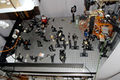
\includegraphics[width=\linewidth,keepaspectratio]{images/120px-MOT_318_t1.jpg}}
  \caption{MOT Optics\\ \href{http://experimentationlab.berkeley.edu/sites/default/files/images/MOT_318_1.jpg}{Click here to see larger picture}}
  \label{fig:MOT_318_1.jpg}
\endminipage\hfill
\minipage{0.24\linewidth}
  \href{http://experimentationlab.berkeley.edu/sites/default/files/images/MOTChamber_284_1.jpg}{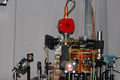
\includegraphics[width=\linewidth,keepaspectratio]{images/120px-MOTChamber_284_t1.jpg}}
  \caption{MOT Chamber\\
  \href{http://experimentationlab.berkeley.edu/sites/default/files/images/MOTChamber_284_1.jpg}{Click here to see larger picture}}
  \label{fig:MOTChamber_284_1.jpg}
\endminipage\hfill
\minipage{0.24\linewidth}
  \href{http://experimentationlab.berkeley.edu/sites/default/files/images/DavLL_289_1.jpg}{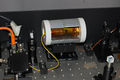
\includegraphics[width=\linewidth,keepaspectratio]{images/120px-DavLL_289_t1.jpg}}
  \caption{DavLL Cell setup\\ \href{http://experimentationlab.berkeley.edu/sites/default/files/images/DavLL_289_1.jpg}{Click here to see larger picture}}\label{fig:DavLL_289_1.jpg}
\endminipage\hfill
\minipage{0.24\linewidth}
  \href{http://dev-physicsadv.pantheon.berkeley.edu/sites/default/files/IMG_4086.JPG}{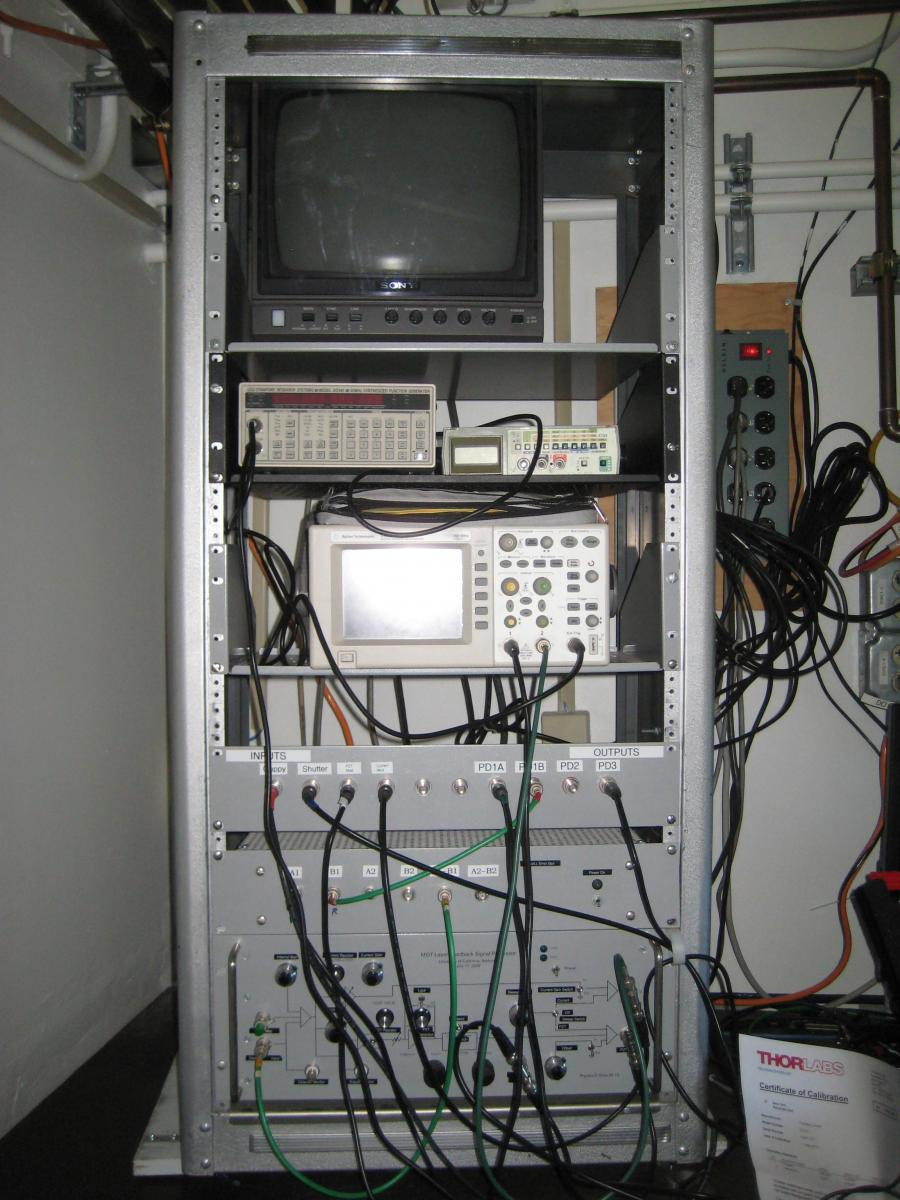
\includegraphics[width=\linewidth,keepaspectratio]{images/IMG_4086.JPG}}
  \caption{MOT equipment rack\\ \href{http://dev-physicsadv.pantheon.berkeley.edu/sites/default/files/IMG_4086.JPG}{Click here to see larger picture}}\label{fig:IMG_4086.JPG}
\endminipage
\end{figure}

\section{Before the 1st Day of Lab}

\textbf{Complete the following before your experiment's scheduled start date:}

\begin{enumerate}
    \item \emph{\textbf{Note: In order to view the private Youtube videos hosted by the university, you must be signed into your berkeley.edu Google account.}}\\
    View the \href{http://youtu.be/1n4QumeydQ4}{\textbf{Atom Trapping Video}}

    \item Before using the apparatus in this experiment, you must complete training in the safe use of lasers detailed on the \href{http://experimentationlab.berkeley.edu/LaserSafety}{\textbf{Laser Safety Training}} page. This includes readings, watching a video, taking a quiz, and filling out a form

    \item Complete the \href{http://experimentationlab.berkeley.edu/MOTPreLab}{\textbf{MOT Pre Lab and Evaluation}} sheets. Print, fill out with the answers and turn it in with your report. The Pre-Lab must be printed separately. Discuss the experiment and pre-lab questions with any faculty member or GSI and get it signed off by that faculty member or GSI. Turn in the signed pre-lab sheet with your lab report.

    \item View the fundamentals of optics tutorial, a review of the principles of optics,\textbf{ }\href{http://experimentationlab.berkeley.edu/sites/default/files/QIE/fundamental-Optics.pdf}{\textbf{\textbf{Fundamentals of Optics Tutorial}}}and the \href{http://youtu.be/zUGBt5vc5FA}{\textbf{Optical Tutorial Video}}, \href{http://youtu.be/wyBOVjU5bBQ}{\textbf{Energy Levels (part 1) Video}} and \href{http://youtu.be/Eypw0DmVBxk}{\textbf{Energy Levels (part 2) Video}}.

    \item \href{http://experimentationlab.berkeley.edu/sites/default/files/MOT/Laser-Guide.pdf}{\textbf{\textbf{View the Laser Guide.pdf }}}and the \href{http://experimentationlab.berkeley.edu/sites/default/files/MOT/Gaussian-Beam-Optics.pdf}{\textbf{Gaussian-Beam-Optics.pdf}}

    \item \textbf{Check points} are examination points that are placed in this lab where you must \textbf{STOP} and call a GSI or professor to make sure you understand what's expected. There could  be multiple check points throughout your lab so make sure you don't skip them since there is a \href{http://experimentationlab.berkeley.edu/checkpointsmot}{\textbf{sign off sheet}} that must be turned in with your lab report. There are 5 Checkpoints in this lab.

    \item Last day of the experiment please fill out the \href{\ExperimentEvaluation}{\textbf{Experiment Evaluation}}
\end{enumerate}

\textbf{Suggested Reading:}

\begin{enumerate}
    \item C. Wieman, G. Flowers and S. Gilbert. ``\href{http://physics111.lib.berkeley.edu/Physics111/Reprints/MOT/MOT\_Plans.pdf}{\textbf{Inexpensive laser cooling and trapping apparatus for undergraduate laboratories}},'' American Journal of Physics \textbf{63}, 317 (1995). Many of the specifics on their experimental setup are different, but they cover the physical and technical concepts of vapor cell MOT's very well.

    \item C. Monroe, W. Swann, H. Robinson, and C. Wieman. ``\href{http://physics111.lib.berkeley.edu/Physics111/Reprints/MOT/Very\%20Cold\%20Trapped\%20Atoms\%20in\%20a\%20Vapor\%20Cell_PhysRevLett.65.1571.pdf}{\textbf{Very Cold Trapped Atoms in a Vapor Cell.}}'' Physical Review Letters \textbf{65}, 1571 (1990). 

    \item \href{http://books.google.com/books?id=hDJPnSFh-g0C&dq=H.J.+Metcalf+and+P.+van+der+Straeten.+Laser+Cooling+and+Trapping+book&printsec=frontcover&source=bn&hl=en&ei=jMWaS4eRD4TuswPgytidAg&sa=X&oi=book\_result&ct=result&resnum=4&ved=0CBAQ6AEwAw#v=onepage&q=&f=false}{\textbf{H.J. Metcalf and P. van der Straten. Laser Cooling and Trapping}} (Springer, 1999). Most directly relevant are Ch. 3 (``Force on two-level atoms''), 7 (``Optical Molasses''), and 11.4 (``Magneto-optical traps''). \href{http://physics111.lib.berkeley.edu/Physics111/Reprints/MOT/Laser\_Cooling\_and\_Trapping\_HJ\_Metcalf/}{\textbf{Searchable PDFs Metcalf Chapters}}

    \item J.J. DiStefano, A.R. Stubberud, and I.J. Williams. \href{http://physics111.lib.berkeley.edu/Physics111/Reprints/MOT/Schaum's\%20Outline\%20Theory\%20and\%20Problems\%20of\%20Feedback\%20and\%20Control\%20Systems/}{\textbf{Schaum’s outline of theory and problems of feedback and control systems online book}}

    \item (McGraw-Hill; New York; 1990). See chapters relevant to frequency-domain analysis of feedback systems.Chapter PDFs \href{http://physics111.lib.berkeley.edu/Physics111/Reprints/MOT/Schaum's\%20Outline\%20Theory\%20and\%20Problems\%20of\%20Feedback\%20and\%20Control\%20Systems/}{\textbf{Searchable chapters 1, 10, 15 16}}
\end{enumerate}

\textbf{Reprints and other materials can be found on the} \href{http://physics111.lib.berkeley.edu/Physics111/Reprints/MOT/MOT\_index.html}{\textbf{Physics 111 Library Site}}

\hyperref[sec:References]{Other References}

You should keep a laboratory notebook. The notebook should contain a detailed record of everything that was done and how/why it was done, as well as all of the data and analysis, also with plenty of how/why entries. This will aid you when you write your report.

\section{Objectives}

\begin{itemize}
    \item Learn what real experimental physics is about

    \item Learn the synergy between experimental and theoretical work

    \item Learn to use pieces of equipment that are commonly used in research

    \item Learn how measurements are performed, analyzed, and interpreted.

    \item Learn how to present your work and results

    \item Learn problem solving strategies

    \item Learn how to manage and organize your time
\end{itemize}

\section{Background}

\subsection{Physics Background}

The operation of a MOT can be understood starting with a few basic principles of atom-light interaction. Here we provide just a sketch of the physics principles involved. A more quantitative treatment, to which you will want to compare your measurements, is found in Ref.~\cite{Metcalf} \href{http://books.google.com/books?id=hDJPnSFh-g0C&dq=H.J.+Metcalf+and+P.+van+der+Straeten.+Laser+Cooling+and+Trapping+book&printsec=frontcover&source=bn&hl=en&ei=jMWaS4eRD4TuswPgytidAg&sa=X&oi=book\_result&ct=result&resnum=4&ved=0CBAQ6AEwAw#v=onepage&q=&f=false}{\textbf{H.J. Metcalf and P. van der Straten. Laser Cooling and Trapping full book}} or \href{http://physics111.lib.berkeley.edu/Physics111/Reprints/MOT/Laser\_Cooling\_and\_Trapping\_HJ\_Metcalf/}{\textbf{Searchable PDFs Metcalf Chapters}}

This description of the operation of a MOT starts with some basic ideas about light-atom interactions and their mechanical effects. We exhibit these basic effects by considering a simple, fictional, ``two-level'' atom. We then consider implications of the specific atomic structure of a real atom, rubidium. Namely, we show how that specific structure allows a MOT not only to cool atoms down to fairly low temperatures (via Doppler cooling), but also to trap them (via Zeeman shifts of optical transitions) while also cooling them to much lower temperatures (via polarization-gradient cooling).

\subsubsection{Scattering Rate}

Let us first consider the absorption and spontaneous emission, or scattering, of light. We focus on just a single optical transition between a particular ground state $|g\rangle$ and excited state $|e\rangle$ of the atom, neglecting for now the complexities of real atomic structure. Such a two-level atom, assumed to have zero velocity, and exposed to monochromatic laser light with frequency $\omega_L$, will scatter photons at a steady-state rate $\Gamma_\text{scat}$ given as
\begin{equation}
    \Gamma_\text{scat} = \frac{\Gamma}{2} \times \frac{s}{1 + s + (2\delta/\Gamma)^2}
\end{equation}
with the following definitions:

\begin{itemize}
    \item $\Gamma$ = the natural linewidth of the transition, given as an angular frequency (units $s^{-1}$) so that $\Gamma^{-1}$ is the lifetime of the excited atomic state.

    \item $s = 2\Omega^2/\Gamma^2$ = the saturation parameter (unitless). We may also express $s = I/I_\text{sat}$ where $I$ is the laser intensity and $I_\text{sat}$ is the saturation intensity.

    \item $\Omega$ = the Rabi frequency (same units as $\Gamma$). This quantity relates to the strength and polarization of the electric field of the laser, and to quantum-mechanical matrix elements that tell us how strongly the ground and excited states of the atom are coupled by laser light. Formally, $\hbar\Omega =  \langle e|d\cdot E|g\rangle$ where $d$ is the electric dipole operator and $ E$ is the laser’s electric field in the co-rotating frame. Clearly, $\Omega^2 \propto  I$.

    \item $\delta = \omega_L - \omega_0$ = the detuning of the laser frequency from the atomic resonance frequency $\omega_0$.
\end{itemize}

\subsubsection{Radiation Pressure}

In a single scattering event, the atom absorbs a photon with momentum $\hbar\vec{k_L}$ from the laser beam, and emits a photon with momentum $\hbar\vec{k_s}$ with the wavevector $\vec{k_s}$ randomly oriented with a probability distribution given by the pertinent dipole emission pattern. Over many scattering events, the average momentum of the emitted photons is zero, giving an average radiation pressure force on the atom:
\begin{equation}
    \vec{F} = \hbar \vec{k}_L \Gamma_\text{scat}
\end{equation}

\subsubsection{Doppler Shift}

In the frame of a moving atom with velocity $\vec{v}$, the frequency of laser light will be different than that observed in the stationary lab frame. The detuning of this light from the atomic resonance frequency will then be given as
\begin{equation}
    \delta' = \delta - \vec{k_L}\cdot \vec{v}
\end{equation}

\subsubsection{Doppler Cooling}

The above ingredients can be combined to explain one of the means, Doppler cooling, by which atoms are slowed down in a MOT from their high velocities in the room-temperature vapor cell to a near standstill. Consider just the one-dimensional motion of an atom in the presence of counter-propagating laser beams with equal frequencies and with wavevectors $k_1 = k$ and $k_2 = -k$, respectively. Summing the radiation pressure from these two beams, we obtain
\begin{equation}
    F = F_1 + F_2 = \hbar k \frac{\Gamma}{2}s\left(\frac{1}{1+s+\left(\frac{2(\delta-kv)}{\Gamma}\right)^2}-\frac{1}{1+s+\left(\frac{2(\delta+kv)}{\Gamma}\right)^2}\right)
\end{equation}
We may expand this equation to first order in the velocity, obtaining $F = -\beta v$. For $\beta > 0$ the radiation pressure provides a damping force to the atoms. In a MOT, atoms are subject to Doppler cooling along all three directions.

\subsubsection{Capture Velocity}
\label{subsubsec:CaptureVelocity}

In a vapor-cell MOT \cite{Monroe}, atoms are captured by laser cooling from high-temperature vapor at temperature . The velocities of atoms in this vapor are nominally distributed according to the Maxwell-Boltzmann distribution,
\begin{equation}
    P(\vec{v}) \propto e^{-mv^2/k_BT}
    \quad \text{or} \quad
    P(v) \propto v^2e^{-mv^2/k_BT}
\end{equation}
While the vast majority of atoms in this distribution are moving far too fast to be slowed effectively by the MOT, atoms in the low-velocity tail, with velocities below a ``capture velocity'' $v_c$, may indeed be captured. We can make a classical estimation of this velocity by considering that the MOT laser beams, with diameter $D$, decelerate atoms with the maximum radiation pressure force of $F_\text{max} = \hbar k \Gamma/2$, giving
\begin{equation}
    v_c \simeq \sqrt{\frac{2F_\text{max}D}{m}}
\end{equation}
From here we can estimate the loading rate of atoms into the MOT as the rate $R$ at which atoms with speeds below $v_c$ pass through the bounding surface of the MOT $\left(\text{area} \propto D^2\right)$, giving
\begin{equation}
    R \propto D^2 \int_0^{v_c} v P(v) \propto D^4
\end{equation}

\subsubsection{Doppler Temperature Limit and Doppler Molasses}

The damping force of Doppler cooling is accompanied necessarily by force fluctuations that prevent the atoms from being cooled to zero temperature. These force fluctuations arise both from the temporally random nature of absorption and spontaneous emission, and also from the random orientation of the emitted photons. As a result of such fluctuations, atoms undergo a random walk in momentum space, with the effect that their momentum variance increases as
\begin{equation}
    \frac{d}{dt}(p^2) = A\Gamma_\text{scat}\hbar k
\end{equation}
where $ A$ is a prefactor of order unity that accounts for the force fluctuations properly. In steady state, the effects of damping and momentum diffusion arrive at a momentum variance characterized by a temperature
\begin{equation}
    T_D = \frac{\langle p^2\rangle}{3 k_B m} = \frac{A}{6}\frac{\Gamma_\text{scat}\hbar k}{\beta}
\end{equation}
The diffusion is also observable in real space: a cold gas of atoms localized initially in the midst of properly tuned counter-propagating laser beams encounters a form of ``optical molasses,'' and will diffuse outwards. You will observe this diffusion in your experiment.

\href{http://physics111.lib.berkeley.edu/Physics111/Reprints/MOT/rubidium85numbers.pdf}{\textbf{\textbf{Data Sheet on Rubidium 85}}}

\subsubsection{Rubidium Spectrum}
\label{subsubsec:RubidiumSpectrum}

\begin{figure}[h]
    \centering
    \href{http://experimentationlab.berkeley.edu/sites/default/files/images/400px-MOTimage005.png}{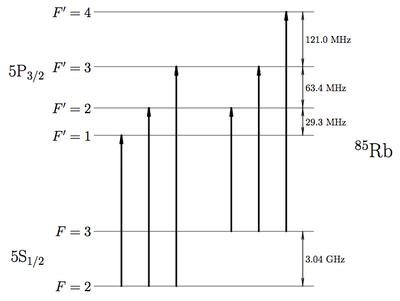
\includegraphics[width=0.6\linewidth]{images/400px-MOTimage005.png}}
    \caption{The energy levels for $^{85}$Rb are shown above with the relative frequency differences between levels. The unidirectional arrows indicate the $D_2$ transition from the 5$S_{1/2}$ ground state to the 5$P_{3/2}$ excited state.}
    \label{fig:400px-MOTimage005}
\end{figure}

To explain the experiment further, it is necessary to move beyond our fictional, two-level treatment of an atom, and to consider instead the real structure and optical properties of atomic rubidium. Rubidium is composed naturally of two stable isotopes, $^{85}$Rb and $^{87}$Rb. In this experiment, we create a MOT for $^{85}$Rb atoms. A pertinent level diagram for $^{85}$Rb is shown in Figure~\ref{fig:400px-MOTimage005} further detail on both isotopes of rubidium is available in Ref.~\cite{Steck}. The transition used for laser cooling drives atoms from the $F = 3$ ground state to the $F' = 4$ excited state of the D2 line. This transition is nominally closed, meaning that atoms will continue to scatter laser light through many absorption/emission cycles. However, rare off-resonant excitation to the $F' = \{2,3\}$ excited states does allow the atom to decay to the $F = 2$ ground state, where it is far-detuned from laser light and thus lost to the laser cooling process. To mend this problem, we introduce also laser light resonant with the $F = 2 \rightarrow F' = 3$ transition, which pumps atoms back to the laser cooled states.

The $F = 3$ and $F' = 4$ levels each contain a number of magnetic sublevels. The strengths of transitions between them are related according to the Clebsch-Gordan coefficients (tabulated in Refs. \cite{Metcalf,Steck}). The strongest transition (lowest saturation intensity) occurs using circular polarized light driving the $|F = 3, m_F = 3\rangle \rightarrow |F' = 4, m_F = 4\rangle$ transition, with $ I_\text{sat} = 1.7$ mW/cm$^2$ \cite{Steck}. In estimating the fluorescence rate of atoms in a MOT, for the purpose of determining the number of trapped atoms, it is suggested that you account for the simultaneous excitation by the many laser beams of the MOT by averaging over all possible atomic ground states and laser polarizations.

\textbf{Effects of the Zeeman shift on light scattering: How a MOT traps}

In the presence of a magnetic field, the energies of the ground and excited state sublevels are shifted by the linear Zeeman shift as $\Delta E = g_F\mu_Bm_FB$, where the Lande g-factors are $ g_F = 1/3$ in the ground state and $ g_F = 1/2$ in the excited state, $\mu_B = h \times 1.4$ MHz/G is the Bohr magneton, $ B$ is the magnetic field strength and the magnetic quantum number $ m_F$ is defined with the quantization axis along the magnetic field direction. These Zeeman shifts vary the atomic resonance frequencies, allowing the radiation pressure force in a MOT to be not only velocity dependent (giving cooling) but also position dependent (giving trapping).

More explicitly, we see that $\sigma^+$ transitions (that increase $m_F$) have higher resonance frequencies than $\sigma^-$ transitions. Given that laser light in a MOT is red-detuned from the atomic transition ( $\delta <0$), we see that a magnetic field will bring the $\sigma^-$ transitions closer to resonance, increasing the radiation pressure force from such light. Now we return to the one-dimensional laser cooling used to explain Doppler cooling and molasses. We consider that both laser beams have left-handed circular polarization; such polarization drives a $\sigma^+$ transition when the laser wavevector points along the magnetic-field axis. Now we consider laser cooling atoms in presence of a linear gradient of the magnetic field, i.e. $\vec{B} = B'z\hat{z}$ (ignoring Maxwell’s equations for now). This configuration ensures that stationary atoms are always forced back to the zero-field position.

In our three-dimensional MOT, we apply gradient fields along all spatial dimensions by creating a spherical quadrupole field, given with Maxwell’s blessing as
\begin{equation}
    \vec{B} = B'z\hat{z} - \frac{B'}{2}(x\hat{x} + y\hat{y})
\end{equation}
The change of sign of the gradient requires that we reverse the laser polarizations of the beams along the $\hat{x}$ and $\hat{y}$ directions.

\subsubsection{Sub-Doppler Cooling}

When researchers carefully measured the temperature of atoms emerging from MOT’s or from optical molasses, they found the atoms were cooled substantially below the temperature limits described by  for Doppler cooling alone. Soon, it was determined that another cooling mechanism, polarization-gradient (PG) cooling, was also at work. Detailed accounts of PG cooling are given in the references \cite{Metcalf}. Here, we provide only a simple explanation of the effect.

PG cooling is based on two phenomena: the AC Stark shift, and optical pumping. The former is a change in the energy of a polarizable object, e.g. an atom, a molecule, or even a glass bead, due to the application of an oscillating electric field. The field induces an electric dipole moment $\vec{d} = \alpha(\omega_L)\vec{E}$ in the object, and then the energy of the object is shifted by the dipole energy $ U = -\vec{d}\cdot \vec{E}$, the time-average of which is non-zero. Here, $\alpha(\omega_L)$ is the dynamic polarizability which, for an atom with a single optical resonance, varies as $\alpha(\omega_L) \sim -1/\delta$. The AC Stark shift is used in many atomic physics experiments to trap ultracold atoms in laser traps. The second phenomenon at work in PG cooling is optical pumping, where light of a certain polarization will define a particular internal state to which the atom will be directed after scattering several photons. Such optical pumping is explored in a \href{http://experimentationlab.berkeley.edu/OPT}{\textbf{separate experiment}} in the 111 laboratory.

In PG cooling, a multi-level atom is subject to AC Stark shifts and optical pumping by light that has a spatially varying polarization. Optical pumping consistently directs the atoms to an internal atomic state in which the AC Stark energy is minimized. However, this pumping does not occur instantaneously. Thus, a moving atom will consistently lose energy as it moves away from the location of minimum energy, as if climbing uphill, only to find itself soon delivered to the bottom of a hill through optical pumping and spontaneous emission. This condition is reminiscent of that of the ancient Greek character Sisyphus, whose punishment for a life of hubris was being commanded to roll a large boulder up a hill, only to watch it roll down again, and to repeat this task eternally.

The end result of PG cooling is the reduction of atomic velocities to temperatures on the order of the AC Stark shift, until one reaches the recoil temperature limit that corresponds to the energy of an atom with just one photon’s worth of momentum.

For completeness, we note that sub-recoil optical cooling is also possible, e.g. through Raman cooling or velocity-selective coherent population trapping. However, these intriguing effects are not relevant to this experiment (at least yet!).

\subsection{Control and Feedback}

(This section as of Fall 2010 is optional)

It behooves the modern physicist to learn about the broad and mature field of control theory; not only does it allow the experimentalist to carry out better experiments but also control theory remains a focus of modern research. There are numerous tutorials on control theory \cite{DiStefano,Dorf,Bechhoefer} to which we refer the interested student. In this experiment, we will explore just a small portion of this field as we set about to control the emission frequency of a diode laser placed inside a low-finesse external cavity \cite{Wieman}. The laser frequency depends on many external influences: the laser current, temperatures of the laser and of the mount structure, the length of the external cavity, the incident angle of light on a diffraction grating within the laser cavity, air pressure, vibrations, etc. To stabilize the laser in the presence of these influences, we use feedback: we measure the emission frequency of the laser, and then make use of two actuators – a piezo-electric transducer (PZT) in the laser cavity and the current supplied to the laser diode – to maintain that measurement at the desired value. Here, we will consider feedback on a linear system, using a frequency domain description (i.e. the frequency at which the laser frequency is varying… perhaps a little confusing). You may have also encountered feedback and control in the BSC portion of the Physics 111 course, where it was presented in the time domain \cite{BSCWriteup}.

\begin{figure}[h]
    \centering
    \href{http://experimentationlab.berkeley.edu/sites/default/files/images/600px-MOTimage001.png}{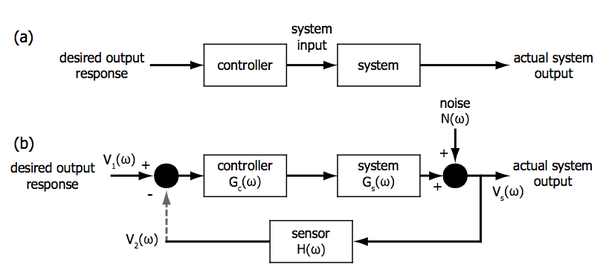
\includegraphics[width=0.9\linewidth]{images/600px-MOTimage001.png}}
    \caption{(a) In a generic control system, a controller translates its input, by which one specifies the desired response of the overall system, to suitable input signals to a physical system. In a feed-forward system, the controller is designed based on a model for the action of the system. Inaccuracies in that model will cause a deviation of the actual system performance from the desired one. (b) In a feedback control system, the system output is sensed and then compared with the desired output; this difference signal is used to adjust the action of the controller. Depending on whether the last link in the system (gray dashed) is connected, the input and output of the overall control system, signals $V_1$ and $V_2$, respectively, are related by the open-loop or closed-loop transfer function. Successful feedback minimizes the difference between $V_1$ and $V_2$, and also suppresses the effects of noise (indicated here by the addition of a spurious signal).}
    \label{fig:GenericControlSystem}
\end{figure}

\subsubsection{Basics}

In a generic control system (Figure~\ref{fig:GenericControlSystem}a), one stipulates a desired output response, e.g. by the input of specific currents or voltages, to a controller device. This controller conditions its inputs to provide a suitable set of parameters to a physical system. This physical system then evolves so as to yield some response, or output. We often think of the controller as a device which the user constructs, with the goal of producing an output response which best matches the desired one. An open-loop control system takes into account only one’s \emph{a priori} knowledge of the response of the system, e.g. based on a well-reasoned physical mode (e.g. consider driving with your eyes closed). As such, this controller is susceptible to modeling errors and changes in the system. In contrast, in a closed-loop control system (e.g. driving with your eyes open), one maintains a prescribed relationship between the desired output and the true system output by comparing them, via a measurement and a comparison device, and using this comparison to drive the controller and system. This feedback lends the control system a much greater robustness and applicability compared to open-loop control.

Our laser system is stable and (approximately) linear, so that the steady-state response of the laser to a sinusoidal system output is a bounded sinusoidal output of the same frequency. For this reason, it is helpful to adopt a frequency-domain picture of the control system. For any component of our control system (e.g. just the physical system, or perhaps the combination of controller, system and sensor), we define the transfer function as $G(\omega) = V_\text{out}(\omega)/V_\text{in}(\omega)$. Here, $V_\text{in,out}(\omega)$ are the input or output at frequency $\omega$, represented as a complex number that describes the phase and amplitude of the signal. These signals need not be measured in the same units; e.g. the input might be a voltage to the laser controller while the output might be the frequency of the emitted laser light, in which case $ G(\omega)$ would have units of MHz/V.

We will find it convenient to represent the gain graphically in two formats. One format is a polar plot, a parametric plot of $G(\omega)$ with $\omega \in \{-\infty, \infty\}$ that defines a contour $\Gamma$ in the complex plane. This method is convenient for ascertaining the stability of a closed-loop system.

Another format is the \href{http://en.wikipedia.org/wiki/Bode\_plot}{\textbf{Bode plot}}, a \emph{log-log plot} of $|G(\omega)|$ and of $\phi = \text{arg}(G(\omega) )$ vs. $\omega$. This plot is convenient in designing a controller than matches well to the system transfer function. We note that the gain is usually plotted in decibels, defined as $ 20\log_{10}|G(\omega)/G_o|$ where $G_o$ is some specified normalization constant; when $G$ is dimensionless, we take $G_o = 1$.

Now consider the feedback control system of Figure~\ref{fig:GenericControlSystem}b. Taking the system as a whole, let’s consider the open-loop response function around the entire control loop, i.e.
\begin{equation}
    G_\text{tot}(\omega) = \frac{V_2(\omega)}{V_1(\omega)} = G_c(\omega)G_s(\omega)H(\omega)
\end{equation}
When the loop is closed and stable, the output $V_2$ responds to variations in the input $V_1$ as
\begin{equation}
    V_2(\omega) = \frac{G_\text{tot}(\omega)}{1+G_\text{tot}(\omega)}V_1(\omega)
\end{equation}
This ratio defines the closed-loop response function of the control system. The control system responds most faithfully with high loop gain at all frequencies.

High loop gain is also beneficial in suppressing the influence of unintended disturbances on system performance. To exhibit this, consider that an unwanted noise signal $N(\omega)$ is added as shown in Figure~\ref{fig:GenericControlSystem}b. While in an open-loop system, $V_s(\omega) = N(\omega)$, upon closing the loop we obtain $V_s(\omega) =\frac{1}{1+G_\text{tot}(\omega)} N(\omega)$, reducing the effect of the disturbance.

\begin{figure}[h]
    \centering
    \href{http://experimentationlab.berkeley.edu/sites/default/files/images/600px-MOTimage002.png}{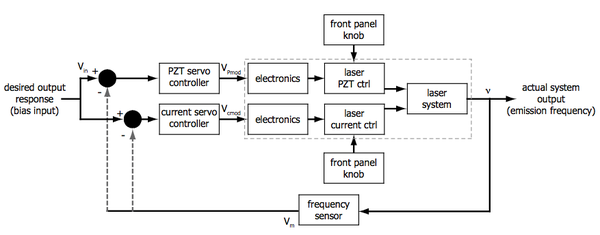
\includegraphics[width=0.9\linewidth]{images/600px-MOTimage002.png}}
    \caption{Laser control system. Two servo controllers are used; one which ultimately controls a piezo-electric transducer (PZT) within the laser housing, and another which controls the diode laser current. The output signals of these controllers, $V_\text{Pmod}$ and $V_\text{cmod}$, respectively, control the ``physical system'' that is the combination of home-built electronics, the electronics within the New Focus laser controller, and the external-cavity diode laser system itself (contents of the dashed gray box). The laser emission is sensed by a laser-spectroscopy setup and a lock-in detection system, yielding a voltage $V_m$ related to the laser frequency. Through this closed-loop system, variations of the bias input lead to controlled variations of the frequency of the laser light.}
    \label{fig:LaserControlSystem}
\end{figure}

\textbf{Conditions for stable feedback}

At some point, however, raising the loop gain makes a system unstable. The condition for stability is stated by the \href{http://en.wikipedia.org/wiki/Nyquist\_stability\_criterion}{\textbf{Nyquist stability criterion}}, which is derived using complex analysis. This criterion states that, considering the contour $\Gamma$ drawn in a polar plot of $G_\text{tot}(\omega)$, a feedback system is typically stable if the contour does not encircle the point ($-$1, 0) \cite{PreciseCriterion}.

This criterion may seem a little too abstract, in which case it might be best just to follow some rules of thumb arising from this Nyquist criterion:

\begin{itemize}
    \item Pay attention to the low-frequency scaling of the open-loop gain. Systems scaling as $G_\text{tot}\propto 1$ (proportional) or $1/\omega$ (an integrator) are likely stable, while those with $1/\omega^3$ or higher scaling are unstable ($1/\omega^2$ is marginal).

    \item One often constructs a feedback system with gain that diminishes with increasing frequency. There, one must pay attention to the frequency $\omega$ where $ G_\text{tot}(\omega) = 1$, the unity-gain point. If $\phi < -\pi$ at this point, the system is likely to be unstable. The quantity $\phi + \pi$ is known as the phase margin – a larger phase margin means your system is more stable to variations (e.g. in the gain). One usually finds that the phase of the system response indeed becomes unmanageable at high frequencies, requiring that one cut off the high-frequency gain (by designing the controller properly) to avoid instabilities.

    \item Resonances in the system induce rapid changes in the gain amplitude and phase, making it hard to guarantee system stability. One usually designs the controller to reduce the loop gain at such resonance frequencies to below unity, avoiding trouble.
\end{itemize}

\subsubsection{Laser Stabilization System}

The laser control scheme implemented in this experiment is diagrammed in Figure~\ref{fig:LaserControlSystem}. This is a two-branch control system, making use of two actuators of the laser system to achieve tighter control over the laser frequency. One of these actuators is a piezo-electric transducer (PZT) that displaces elements within the laser cavity. The PZT is useful for scanning the laser frequency stably over a very broad range, and, thus, is controlled by an integrator which allows the laser to compensate for long-term drift in its emission frequency. However, as you will see, the useful bandwidth of the PZT actuation is limited. Thus, high frequency feedback is achieved by a different actuation mechanism, a variation of the current supplied to the laser diode. The overall transfer function for this control system is the sum of the responses of the two feedback branches.

\section{Safety}

In working with this experiment, you must be mindful of a few hazards.

\begin{itemize}
    \item \textbf{Laser light}: This experiment uses a $\sim$50 mW beam of laser light at a wavelength of 780 nm. This light is infrared, beyond the range of human vision except for very bright illumination. Such a Class IIIb laser may damage your eye both from direct viewing and from diffuse scattering. Thus, you must wear laser safety goggles (provided in the laboratory) once the curtain around the table is drawn open. To align optics or search for stray laser light, you should use a fluorescent laser viewing card or an IR scope. Be particularly careful working near the vacuum chamber, where there are vertically oriented beams and also horizontal beams at several elevations.

    \item \textbf{High voltage}: The ion pump is supplied with high voltage for its operation. While the cabling for this ion pump leaves no high-voltage connection exposed, you should not touch or modify the ion-pump setup; rather, ask a professor or teaching assistant for help.

    \item \textbf{Ultra-high vacuum}: You must be careful not to drop anything on the glass viewports of the vacuum chamber. If they break, not only will your experiment be ruined, but also the imploding glass can be hazardous. If you must use a metal tool near those viewports, consider blocking the glass windows in case the tool slips from your hands.
\end{itemize}

\section{Equipment used in this experiment}

\begin{enumerate}
    \item Ion Pump; Never turn off

    \item Ion Gauge; to read the pressure in the chamber, Leave on

    \item Rubidium chamber Getter and controls (use power supply \#1)

    \item Rubidium metal sample; back up source of Rubidum (Not used normally)

    \item Turbo Pump and roughing pump with LN-2; Used only by staff if vacuum fails Read the Cryogenic Safety sheet: See the Cryogenic Liquids information from EH\&S \href{http://experimentationlab.berkeley.edu/sites/default/files/SHE/77cryogenic.pdf}{\textbf{Cryogenic Training}}

    \item Video Camera to view Atoms in chamber

    \item Gumpy Trigged CCD Camera to measure number of Atoms, etc and controlled by the LabView Program

    \item Laser 780nm 45mW split into three beam paths X,Y,Z

    \item Optical Isolator

    \item IR Viewer; to view beams which are invisble puls IR cards to view beam directly

    \item Safety Goggles wear at all times when Laser in operation

    \item Digital Scope;

    \item \href{https://youtu.be/PrM8DHFOFS0}{\textbf{SR345 Function Generator}}

    \item Physics 111-Lab Laser Lock-Box and Feedback control

    \item Error amplifier

    \item DAVLL Cell

    \item Optical Detectors

    \item Lens, Mirrors, 1/4λ plates

    \item Ghz Frequency meter

    \item VCO signal

    \item Heater controllers
\end{enumerate}

\section{Experimental Setup}

\subsection{Optics}

\begin{figure}[h]
    \centering
    \href{http://experimentationlab.berkeley.edu/sites/default/files/images/800px-Setupv7.png}{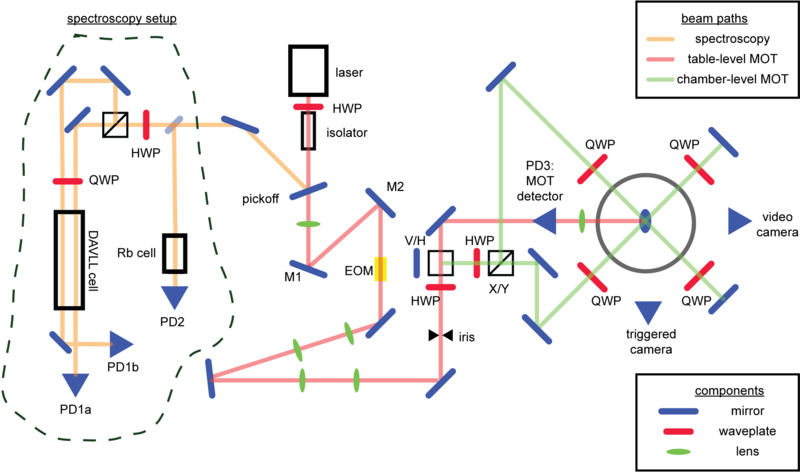
\includegraphics[width=0.6\linewidth]{images/800px-Setupv7.png}}
    \caption{Optical Setup for the MOT experiment}
    \label{fig:OpticalSetup}
\end{figure}

\subsection{Standard Operating Procedures (SOP) and MOT Optics}

\begin{itemize}
    \item Note you need 80 PSI water pressure. Look at the prssure meter on the south wall behind the computer and see that is at 80 PSI.
    
    IF not see Don Orlando immediately.

    \item Before turning on the laser, examine the optical table for misplaced objects in the laser beam path. Refer to Figure~\ref{fig:OpticalSetup} for a reference diagram. You may want to print out a copy of this diagram. Once the path is clear, \textbf{put on a pair of the Laser Safety Goggles} and turn on the laser. Adjust the current to around 100 mA. Laser light emerges from a commercial diode laser (New Focus Stablewave) with linear polarization.

    \item Now check for stray beams: You should perform a survey of the laser beam paths to check if there are any stray beams (diffuse or specular) emanating from any part of the laser path and its optics. Then document this in the Laser Log Book in the wall pocket near the apparatus. Make sure that the shutter is open as you follow the beam path around the optical table. (currently using shutter \#2) Toggle switch to N.O. to open it, the main power switch is on the back of unit. The laser safety survey is done by using the IR Viewer and a white piece of paper or business card. If the IR Viewer is not in the room, ask a staff person to locate it. The IR viewer is blue in color and you use it with your goggles on. Using the paper card follow all of the beam paths from the laser to the vacuum chamber and from the laser through the spectroscopy setup section (see Figure~\ref{fig:OpticalSetup}). Note if the beam strays from its intended path. It should go through the lenses and reflect from mirrors, but should NOT hit or reflect off of anything else (including the mounts) on the optical table. This laser beam is hazardous to your eyes if they are un-protected as you cannot see the laser light. Keep the goggles on at all times for your safety.

    \item The \href{http://en.wikipedia.org/wiki/Optical\_isolator}{\textbf{optical isolator}} minimizes the reflection of light back into the laser from the optics on the table. Such reflections can destabilize the laser, essentially turning the whole table into a laser resonator. You may see such instabilities when light from the MOT beams is retro-reflected into the laser, in which case the staff may want to adjust the optical isolator. A \href{http://en.wikipedia.org/wiki/Wave\_plate}{\textbf{waveplate}} before the resonator adjusts the linear polarization to match the input polarizer of the isolator.

    \item A pickoff beam-splitter sends some of the light toward the rubidium spectroscopy system.

    \item The \href{http://en.wikipedia.org/wiki/Electro-optic\_modulator}{\textbf{electro-optical modulator}} (EOM) is a non-linear optical crystal placed within a tuned microwave resonator. A resonant microwave signal creates a strong time-varying electric field that distorts the crystal and varies its index of refraction. The laser beam, passing through that varying index material, becomes phase modulated at the frequency of the microwave input. In this manner, we add frequency sidebands to the laser, shifting some of the laser power (a few percent) to a frequency that will repump atoms on the repumping transition. The EOM crystal is birefringent, and its refractive index varies only for one linear polarization. The waveplate after the isolator rotates the polarization appropriately. Further details on this EOM are available in the \href{http://physics111.lib.berkeley.edu/Physics111/Reprints/MOT/Modulators.pdf}{\textbf{EOM 4431 Data Sheet}}.

    \item Several lenses act as a telescope to expand and circularize the beam. The beam should be aligned through the center of and parallel to all these lenses.

    \item A variable iris sets the diameter of the laser beams. Using the IR viewer and viewing the input face of the iris, you should see that the laser beam is reasonably well centered on the iris.

    \item We use half-wave plates and polarizing beam cubes to split the optical power between the different MOT beams. The H/V splitter divides between the horizontal and vertical beams, while the X/Y splitter divides between the two horizontal beams.

    \item On each of the three MOT beams, light passes first through a quarter-wave plate. When rotated to the correct position, this waveplate converts the incoming linear polarized light to circular polarization of the correct helicity for the operation of the MOT. After passing through the vacuum chamber, the beams pass another quarter-wave plate and are retro-reflected.

    \item The many mirrors in the optical path are placed there intentionally so that the optical system can be adjusted to match its many constraints. For example, we highlight two mirrors (M1 and M2) before the EOM. These two mirrors are used to align light through the EOM. This alignment must satisfy four constraints: we require that the beam enter the EOM near the center of the input facet (a specific location in 2D, giving two constraints) and exit near the center of the output facet. The two mirrors before the EOM have four degrees of freedom – the horizontal and vertical tilts – matching the number of constraints. These mirrors should be aligned iteratively to satisfy the alignment constraints, a procedure known as ``walking the beam.'' \cite{SUNYStonyBrook}. This mirror arrangement is known as a ``dog-leg,'' and is repeated throughout the optical setup.
\end{itemize}

\subsubsection{Rubidium Spectroscopy Setup}

Now we return to the optical setup where a rubidium vapor is probed in order to determine the frequency of the laser with respect to the rubidium resonance lines.

\begin{itemize}
    \item Following the beam pickoff, light is divided again into two beams.

    \item The first beam passes through a glass cell containing a dilute Rb vapor before being sent to photodetector PD2. In this arrangement we obtain Doppler-broadened features (four broad absorption peaks -- you should explain what these are). We use these features as frequency markers by which to interpret the error signal obtained from PD1a and PD1b.

    \item The second beam is used for a Dichroic Atomic Vapor Laser Lock (DAVLL) setup \cite{Corwin}. We use this cell with Rb vapor, to which a near-constant magnetic field, oriented along the direction of laser propagation is applied using a pair of permanent magnets. Two beams of orthogonal linear polarization enter at slightly different points in the cell with a polarization beam splitter. At the input of the cell, a quarter-wave plate is used to measure the laser power in the two circular polarizations, $\sigma^+$ and $\sigma^-$, on the two photodetectors PD1a and PD1b, respectively. As explained below, taking the difference between these two photodiode signals gives us a measure of the frequency of the laser, which we use for feedback stabilization.
\end{itemize}

Let us now describe briefly the origin of the signals seen on the three photodetectors. Neglecting first the effect of light polarization and of an applied magnetic field, a laser beam passing through the Rb vapor cell will be partly attenuated due to the absorption and rescattering of light by the Rb atoms within the cell that experience the laser light frequency as coinciding with an atomic resonance. Recalling that the atomic vapor inside the cell contains atoms with a thermal distribution of velocities, laser light at detuning $\delta$ with respect to the resonance frequency $\omega_o$ of a stationary atom will be absorbed by atoms with velocity $ v = -\delta/k_L$ along the laser propagation direction, i.e. by a fraction $ P(v) \propto  e^{-m v^2/k_B T}$ of the vapor. Light exiting the cell is attenuated by a factor $ t = e^{-OD(\delta)}$ (Beers’ law) where the optical density $ OD$ is proportional to $P(v = -\delta / k_L)$ and also increases with increasing Rb vapor pressure as you heat the cell. Thus, because the atoms in the cell have a large velocity variance, significant absorption occurs over a wide range of laser frequencies.

Now, from the discussion on the \hyperref[subsubsec:RubidiumSpectrum]{rubidium spectrum}, the atomic resonance frequencies for $\sigma^+ $ and $\sigma^- $ polarized light are shifted differentially in an applied magnetic field, causing the Doppler-broadened absorption line to be shifted upward in frequency for one circular polarization and downward in frequency for the other. The gas now displays circular dichroism, meaning that the absorption is generally different for the two circular polarizations. Taking the difference in the measured transmitted laser powers for the two circular polarizations provides a signal which crosses zero and varies linearly near the peak of the zero-field Doppler absorption profile. This signal is then suitable for stabilizing the laser frequency near that absorption peak.

\subsection{Vacuum System}

\begin{figure}[h]
    \centering
    \href{http://experimentationlab.berkeley.edu/sites/default/files/images/500px-MOTimage008.png}{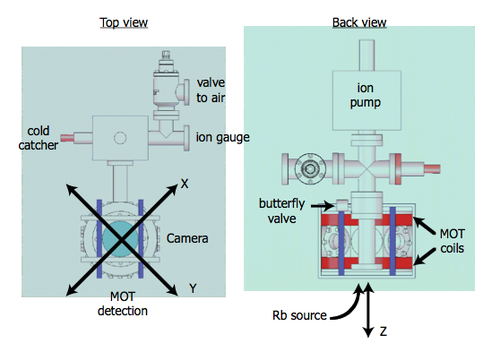
\includegraphics[width=0.5\linewidth]{images/500px-MOTimage008.png}}
    \caption{Vacuum chamber details.}
    \label{fig:VacuumChamberDetails}
\end{figure}

The MOT is created at the center of an evacuated, octagonal vacuum chamber graced with many glass viewports to allow laser light to be directed at the atoms, and surrounded with electromagnets to create the requisite magnetic field. Follow along as we describe the elements of the vacuum apparatus, illustrated in Figure \ref{fig:VacuumChamberDetails}.

\begin{itemize}
    \item You will be using an electronic rubidium getter to supply the MOT cell with rubidium via power supply \#1. As a backup (which will only be used by laboratory staff if necessary), a chunk of rubidium, with natural abundances of $^{85}$Rb and $^{87}$Rb, rests at the bottom of a flexible vacuum tube. This metal emits a low-pressure vapor of atomic Rb. The temperature of the bottom flange of this tube is controlled by a thermo-electric cooler (TEC), one face of which is connected to the flange, and the other face of which connects to a water-cooled copper plate. This temperature is monitored and maintained by a controller located above the MOT optics. The TEC may be supplanted by a band heater in case you need to heat the rubidium source a lot to get a reasonable vapor in the chamber. However, the current for the Rb chamber getter should not exceed 5 Amps, so please don't overheat the rubidium without consulting with the laboratory staff. Too much Rb vapor can mess up the vacuum system and require a lengthy vacuum bakeout. See Don for help!

    \item The pressure of Rb and other gases in the chamber is controlled by a pumping system comprising a butterfly valve, which restricts the pump speed, a TEC-cooled in-vacuum plate, upon which Rb vapor condenses, an ion pump, and a turbo-molecular pump backed by a roughing pump.

    \item To understand the order in which the pumps operate, consider when the chamber is at atmospheric pressure. The roughing pump is used to pump until the chamber has a pressure of approximately 40 millitorr. Beyond this point, the roughing pump is ineffective, so the turbo pump takes over and gets the chamber to $10^{-8}$ torr. While very powerful, the turbo pump is also very delicate, so once it is finished it turns off and disconnects from the vacuum system. The ion pump then takes over and maintains the vacuum. The vacuum pressure may be read out from the ion pump gauge, which is located below the optics table. You should not need to adjust the pumping station – ask for help if you suspect something is wrong.

    \item For a more in-depth explanation to vacuum technology, please consult Ref.~\cite{Moore}.

    \item The octagonal chamber is surrounded by several electromagnet coils. A large set of coils (MOT coils) generates the spherical quadrupole field required for the MOT. These coils are wired so that top coil (or, actually, a set of connected layers of coils) runs current in a sense opposite to that of the bottom coil. The coils, made of hollow copper tubing through which we run water, are supplied with up to 100 amperes of current by a current supply located below the optical table. Several other sets of coils (field coils) generate nearly uniform fields in three cardinal directions, and are supplied by additional supplies below the table. These coils are not used in the present version of this experiment.
\end{itemize}

\subsection{Electronics for Laser Stabilization}

Let us familiarize ourselves with the electronics used to control the laser and implement feedback. A simplified diagram of the servo controller is provided in Figure~\ref{fig:SchematicOfServoController}. The \href{http://experimentationlab.berkeley.edu/sites/default/files/images/Full\_schematic.pdf}{\textbf{full-blown schematic}} contains further details, e.g. on the notch filter and adding circuits.

\begin{figure}[h]
    \centering
    \href{http://experimentationlab.berkeley.edu/sites/default/files/images/Electronics_schematic_v2.png}{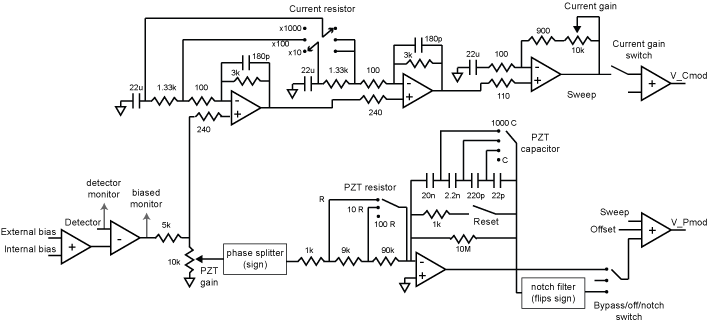
\includegraphics[width=0.7\linewidth]{images/Electronics_schematic_v2.png}}
    \caption{Schematic of the servo controller. Input: A bias voltage is taken as the sum of an externally provided voltage and an internal variable voltage and is then subtracted from the detector input. Buffered monitors give the detector voltage before and after that subtraction. PZT branch: Following a variable voltage divider, to set the overall PZT feedback gain, the signal is sent through a circuit that can flip its sign. Next, an op-amp with variable input resistors and feedback capacitors determines the PZT feedback gain. A switch selects between the direct output of this op-amp, ground (switching off the PZT gain), or a notch-filtered (and inverted) version of the op-amp output. The voltage is then summed with the external sweep and a manually dialed offset voltage. Current branch: A two-op-amp circuit establishes the gain settings for the current feedback, with a rotary dial establishing three different gain settings. The signal is sent through another amplifier with variable gain. Following the current gain on/off switch, the signal is then added to the external sweep and output.}
    \label{fig:SchematicOfServoController}
\end{figure}

\subsection{Rubidium Getters}

A rubidium getter is comprised of a stainless steel oven, which contains several milligrams of rubidium. Several of these ovens are then affixed to the pins of a vacuum feedthrough system. When current is applied (3-5 A) to the oven, the rubidium heats up and produces a vapor, which then enters the vacuum chamber. The more current is applied, the more rubidium vapor will be produced and flow into the chamber. See Don for Help!

\begin{figure}[h]
    \centering
    \href{http://experimentationlab.berkeley.edu/sites/default/files/images/MOT_Rb_getters2.png}{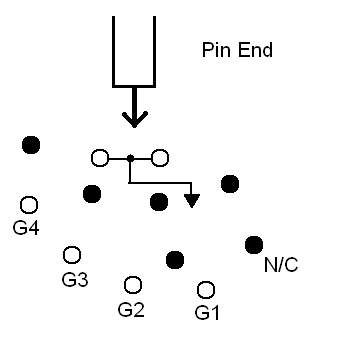
\includegraphics[width=0.35\linewidth]{images/MOT_Rb_getters2.png}}
    \caption{Diagram of the pins of the vacuum feedthrough system and their corresponding Rb getters. The open circles represent pins that are connected, while the solid circles are not connected to any getters.}
    \label{fig:MOT_Rb_getters2}
\end{figure}

\section{Procedure}

\subsection{Overview and time-line}

The experiment is divided into two main portions (and should be completed roughly according to the following schedule). The first half requires you to stabilize the frequency of a diode laser system \textbf{(Days 1-3)}. The goal of the second portion is to produce a stable MOT \textbf{(Days 3-4)} and provide qualitative and quantitative assessments of its characteristics \textbf{(Days 4-5)}.

\subsection{Task 1: Understanding Your Laser and Vacuum System}

Your first task is to familiarize yourself with the equipment. As you read through the following description, you are asked to identify and start working with the various experimental components.

Before you leave each day, make sure to review the MOT equipment list (below) for details on which devices should be turned off and which should be powered on. This is incredibly important, as failure to turn off some equipment could damage the system permanently.

\textbf{LEAVE ON THE FOLLOWING EQUIPMENT:}

\begin{itemize}
    \item Rb small Cell Heater power(under table)

    \item Ion Pump controller (under table)

    \item Ion Gauge Controller (under table, pressure should be about $4 \times 10^{-8}$ torr)

    \item VCO Box (above table)

    \item Rb DAVLL Cell heater power (above table)

    \item Cold Trap Power (above table)
\end{itemize}

\subsubsection{MOT Optics To do:}

The optical setup for this experiment is, at first glance, rather complex, comprising many lenses, mirrors and other optical components, and possessing very many knobs with which to adjust and tune the optics. To understand the role of and relation between all these components, it is best to use an IR viewing card and to follow the path of laser light through the apparatus.

As you go through the optics and learn about what all the components do, you will be tempted to tweak the setup and see what happens. You should feel free to do so, but it would be wise to take note of what you are doing, and to return the setup to its original configuration when you are done with your tweaking, at least until you feel very confident that you know you are doing the right thing (say on the last day or two of the lab). Otherwise, you will find yourself trying to improve the optical setup but only making it more misaligned and poorly performing.

\begin{itemize}
    \item Measure the optical power along the different beam paths. Repeat these measurements throughout the experiment to diagnose problems as they arise.

    \item At what frequency should the EOM be driven? Use a frequency meter to monitor the pre-amplifier microwave signal to see that the drive frequency is appropriate. Note also that the EOM has a narrow resonance; if you send in a microwave signal at the wrong frequency, that signal is reflected and directed, after attenuation, to the post-amplifier port of the microwave signal box. A hand-held frequency meter (a little black box from Elenco) provides a rough measurement of that reflected power (look for the signal bars below the frequency reading... and don't worry about the frequency reading, as it's outside the range for which the Elenco device is reliable). Tune the EOM input frequency to minimize this reflected power and note the center and width of the EOM resonance. If the EOM resonance seems to be at a microwave frequency far from what you need for the MOT, the EOM might need tuning. Ask a staff member for help.
\end{itemize}

[NOTE: As of April 13, 2010, the following settings of the rotatable quarter wave plates should give the proper circular polarization for a MOT: X-axis, rotation stage at 20 with numbers facing the incident beam; Y-axis, rotation stage at 268 with numbers facing the incident beam; Z-axis, rotation stage at 0 with numbers facing up]

\textbf{(2 Signatures) This is a checkpoint and a great time to stop and think about the physics at play. Discuss the following questions with you partner and once you feel you have a better understanding of what is happening, call over a GSI to sign you off:}

How does the power coming from each output port of the beamsplitter change as the preceding waveplate is rotated? Explain this quantitatively.

Explain how the two quarter-wave plates on the chamber level MOT beam path should be adjusted to provide the correct helicities for the operation of the MOT. What happens to the light polarization when the waveplates are rotated? Why is there no rotator on the second waveplate?

\subsubsection{Vacuum Chamber To Do}

\begin{itemize}
    \item Monitor the vacuum pressure using the ion gauge (located under the MOT optics table) and keep note of it during the experiment. Be sure you understand what the reading means. However, you should not need to adjust the pumping station – ask for help if you suspect something is wrong.

    \item Calculate the magnitude of the field gradient (as defined in ) produced by a 1 A current running through the MOT coils. For this, note that the top MOT coil consists of three layers with 15 turns each, and that the MOT current runs \emph{in series} through these three layers; same for the bottom coil.
\end{itemize}

\subsubsection{Rb Spectroscopy To Do}

\begin{itemize}
    \item Considering a single atomic transition in Rb, what absorption rms linewidth (in MHz) do you expect due to Doppler broadening in the small Rb cell (which is kept near room temperature)? Remember the Doppler shift is sensitive only to one components of the velocity vector.

    \item Using an IR viewer card, estimate the diameter of the beams used in your Rb saturation spectroscopy setup as it enters the vapor cell. How much power do you need in that beam to reach the saturation intensity for Rb (say at the center of the beam profile)? Now measure the power in the beam using the power meter, and confirm that the power is sufficient.
\end{itemize}

\subsection{Task 2: Generating and Calibrating an Error Signal}

Your next task is to generate absorption spectra for the relevant Rb lines and derive an error signal to use for laser stabilization. Please reference the experimental setup portion of this manual for a circuit block diagram. The laser controls are listed and described below.

\subsubsection{Inputs}

\begin{itemize}
    \item \textbf{DETECTOR INPUT}: Input to both the PZT and current servo controllers. In the closed feedback system, this input comes from your laser frequency measurement.

    \item \textbf{EXTERNAL BIAS}: This signal is subtracted from \textbf{DETECTOR} to generate the error signal. When the feedback system is closed, the laser frequency effectively follows this input. ''\emph{NOTE: In the present version of this experiment, you will not be using this port, so just ground it with a terminator.}

    \item \textbf{SWEEP INPUT}: This input is multiplied by a user-set scale factor (\textbf{SWEEP GAIN}) and then added into either the \textbf{PMT MOD} or \textbf{CURRENT MOD} output. It is used to scan the laser frequency in order to located and analyze the Rb spectroscopy signals, and also to zero in on the desired lock point. The function generator will feed into the circuit until the laser is locked.
\end{itemize}

\subsubsection{Front panel controls}

Input stage:

\begin{itemize}
    \item \textbf{INTERNAL BIAS}: This controls a constant analog voltage that is also subtracted from the \textbf{DETECTOR INPUT} signal. Useful for dialing around the laser setpoint when the system is locked.
\end{itemize}

PZT feedback branch:

\begin{itemize}
    \item \textbf{PZT GAIN}: A 10-turn trimpot adjusts the overall gain of the PZT feedback branch.

    \item \textbf{POLARITY}: A switch changes the sign of the feedback.

    \item \textbf{PZT RESISTOR}: A three-position dial varies the input resistor on the op-amp used for feedback.

    \item \textbf{PZT CAPACITOR}: A four-position dial varies the capacitor on the feedback branch of the op-amp.

    \item \textbf{RESET}: Switches the low-frequency PZT feedback between being an integrator and having proportional gain. Down means the integrator is off.

    \item \textbf{BYPASS/OFF/NOTCH}: There is a notch filter to extinguish the response of the PZT feedback around the resonance frequency of the PZT (around 2.4 kHz). This is a three-pole switch, for which the settings are: up = notch is bypassed, PZT feedback is on; middle = PZT feedback is off; down = notch is used, PZT feedback is on.

    \item \textbf{OFFSET}: You can add a constant voltage to the PZT output, controlled by the offset knob and switch.
\end{itemize}

Current feedback branch:

\begin{itemize}
    \item \textbf{CURRENT RESISTOR}: A three-position dial that controls the magnitude of the current gain.

    \item \textbf{CURRENT GAIN}: Controls the current gain.

    \item \textbf{CURRENT GAIN SWITCH}: switches the current gain on/off.
\end{itemize}

Sweep:

\begin{itemize}
    \item \textbf{SWEEP GAIN}: Varies the strength of the sweep.

    \item \textbf{SWEEP SWITCH}: A three-pole switch that selects whether to send the sweep input onto the current modulation (up), the PZT modulation (down), or to neither output (middle). \emph{NOTE: Even in the middle position, there is a small ($\sim$part in a thousand) contamination of the sweep input onto the PZT and current modulation that can affect the stability of the laser. When you're not using the sweep, you might want to disconnect the sweep input or at least set the amplitude of the sweep to zero.}
\end{itemize}

\subsubsection{Outputs}

\begin{itemize}
    \item \textbf{PZT MOD:} Control signal sent to the laser controller through a 10:1 voltage divider to vary the PZT setting in the laser head.

    \item \textbf{CURRENT MOD:} Control signal sent to the laser controller to vary the current supplied to the laser.

    \item \textbf{DETECTOR MONITOR}: A low-pass, buffered replica of \textbf{DETECTOR INPUT}. When the laser is locked with the integrator, you can read this signal to determine what is the laser frequency according to your prior calibration.

    \item \textbf{BIASED MONITOR}: A low-pass, buffered replica of the error signal after the analog \textbf{INTERNAL BIAS} and \textbf{EXTERNAL BIAS} have been subtracted out. When the system is locked with the integrator, this output should be near zero.
\end{itemize}

\subsubsection{Generating the error signal}

\emph{Observe the Doppler-broadened absorption spectrum:}

\begin{itemize}
    \item Input a low-frequency sweep (triangle wave, 10’s of Hz) from the SRS DS345 generator into the \textbf{SWEEP INPUT} port of the laser controller and direct the sweep (using the front-panel switch) to the PZT output. We use a triangle-wave so that the variation in the PZT voltage is linear in time, making it easier to interpret the signals on the scope. Be mindful that the PZT will ring slightly at the ends of your triangle-wave sweep; we mitigate that problem somewhat by sweeping very slowly.

    \item Now monitor the output of the spectroscopy setups on a scope as you vary the offset voltage, either on the servo controller or the laser controller. For this, you may want to use the DS345 SYNC output to trigger the scope.

    \item Expand the sweep range so that you see four broad dips in the transmission through the spectroscopy setup (PD2). The hyperfine splitting of the excited state is unresolved for the Doppler broadened signals. Look up \cite{BSCWriteup,Steck} and identify these with the four ground-state hyperfine manifolds of $^{85}$Rb and $^{87}$Rb. Note the frequency splitting between these Doppler-broadened absorption lines. You can now monitor the \textbf{PZT MOD} signal on the scope (using a BNC Tee), and thus make a first determination of the low-frequency transfer function (MHz/V) of the PZT controller.  Later on, when you focus on the DAVLL error signal right around the line used for laser cooling, you will use this transfer function to know how to relate the voltage of your error signal to the frequency offset of the laser.
\end{itemize}

\begin{figure}[h]
    \centering
    \href{http://experimentationlab.berkeley.edu/sites/default/files/images/400px-RbSpecMOT.GIF}{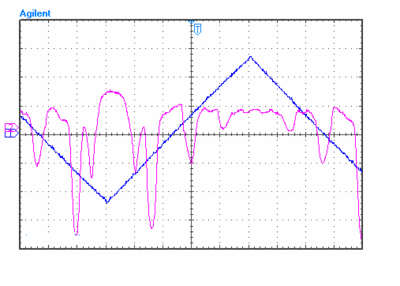
\includegraphics[width=0.5\linewidth]{images/400px-RbSpecMOT.png}}
    \caption{A sweep of the 4 Rb spectrum lines as will be seen on the scope along with the sweep of the function generator. Notice the mirroring on the down sweep.}
    \label{fig:400px-RbSpecMOT}
\end{figure}

\textbf{This is a checkpoint and a great time to stop and think about the physics at play. Discuss the following questions with you partner and once you feel you have a better understanding of what is happening, call over a GSI to sign you off:}

Once you get your response from the photodetector as the picture shown above show your GSI the signal on the scope and point at the four peaks that correspond to the two different states of Rb$^{85}$ and Rb$^{87}$ respectively (don't forget to mention which transition is which).

Note that the digital storage scope used for this experiment is connected to a computer, so that you can record data for analysis and your lab report.

\emph{Obtaining the DAVLL signal:}

\begin{itemize}
    \item Turn on DAVLL heater and leave it on. The heater should reliably supply rubidium into the cell at 1 volt and 4 amps, slight adjustments should not be necessary. Do not exceed 5 Amps without consulting the laboratory staff.

    \item Narrow the sweep onto the $^{85}$Rb $F=3 $ and the $^{87}$Rb $F=2 $ absorption lines. You should see the rubidium fluoresce within the beam paths on the video monitor. Examine both the spectroscopy signal (PD2) and the DAVLL signal (PD1a-PD1b) simultaneously. Now, block each of the two DAVLL-setup photodiodes in turn. You should see the Rb-cell absorption lines for $\sigma^+ $ and $\sigma^-$ laser light, respectively (recall that you're looking at the output of a difference op-amp circuit, the DAVLL error box, PD1a-PD1b signal). Ignore this next sentence: Notice that the line centers of these different absorption lines are shifted from the field-free lines seen in the saturated absorption cell. From this difference, determine what is the magnetic field inside the DAVLL vapor cell.

    \item Now allowing light into both PD1a and PD1b, you should see the DAVLL error signal. Explain why it has the form that it does.

    \item Center and then narrow the sweep onto the $F = 3 \rightarrow F' = 4 $ transition. You may take some time to optimize this error signal; for our purposes, we want the detector signal to have a large slope and also to cross zero near the center of the transition. Consider varying the settings of the two waveplates in the DAVLL set up, the temperature of the DAVLL vapor cell (but notice that this temperature takes a long time to settle), and the alignment of the two photodiodes (as a last resort).
\end{itemize}

\begin{figure}[h]
    \centering
    \href{http://experimentationlab.berkeley.edu/sites/default/files/images/400px-Rb3to4withErrorAC.GIF}{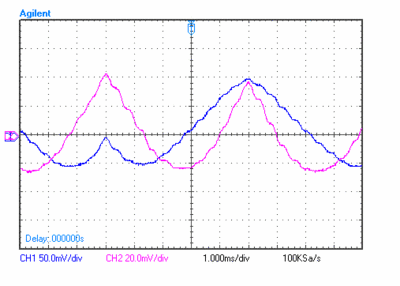
\includegraphics[width=0.5\linewidth]{images/400px-Rb3to4withErrorAC.png}}
    \caption{Digital Scope Output of a working MOT near the Rb 85 3 to 4 transition. Pink line is PD2 and the blue line is an example output of biased monitor DC coupled. Notice that it is linear and crosses the zero near the center of the peak.}
    \label{fig:400px-Rb3to4withErrorAC}
\end{figure}

Ignore paragraph below

\emph{Calibrating the locking signal:}

\begin{itemize}
    \item You will want to know how to relate the voltage of the locking signal to the frequency of your laser. For this, you need some well defined frequency references by which to calibrate the signal. These references are provided by the saturated absorption signal recorded on PD2. Identify the narrow absorption features observed on PD2. For each of these features, record the PZT control voltage and also use spectroscopic data (e.g. Ref.~\cite{BSCWriteup}, Table 1). From these, you should obtain a linear frequency scale to which to calibrate your locking signal. We suggest you measure frequency in terms of the detuning from the $^{85}$Rb cycling transition, and approximate your error signal as linear near $\delta = 0$. Note: you may need to repeat this calibration procedure several times during this lab.
\end{itemize}

\subsection{Locking the Laser}

\subsubsection{Measuring the system transfer functions}

The linear relation obtained while calibrating the locking signal gives the sensor transfer function $ H(\omega)$ (in units of V/MHz) for low-frequency modulation of the laser. The next step in designing our servo system is to determine the system transfer function $ G_s(\omega)$ for both the PZT and current transducers. To do this, first set the PZT offset voltage so that a frequency scan on either the PZT or current inputs will be centered near $\delta = 0$, on the linear portion of the DAVLL signal. To determine $ G_s(\omega)H(\omega)$ (dimensionless units), use the DS345 generator to produce a zero-offset sine-wave modulation that drives \emph{either} the PZT or current controller. Observe both the sinusoidal drive (using a BNC-T at the PZT or current controller input) and also the DAVLL signal on the oscilloscope. Record both the magnitudes of the two voltage modulations and also the phase offset between them. You will find this is easiest to do using the ``Measure'' function on the oscilloscope, by which you can obtain determinations of the peak-to-peak voltage of both channels and also the temporal delay between them. From these data, you should produce Bode plots for both the PZT and current branches.

For the PZT branch, record the gain between DC and $\sim$10 kHz. You will notice many resonances in this record. Take data with sufficient resolution to characterize the two lowest-frequency resonances in detail (starting near 2 kHz). These resonances are both electronic and mechanical. For the remaining resonances, just record their resonance frequencies. For the current branch, record the gain between DC and 1 MHz. Confirm that the response is fairly featureless. As you take these data, keep adjusting the amplitude of the sweep input so that the locking signal stays within its linear range. Be particularly careful not to drive the system too hard at its resonances, so as not to damage the laser.

\subsubsection{Tuning the lock box}

Now we can design the servo system to lock the laser frequency with high loop-gain and without oscillating. First consider the PZT branch.

\begin{itemize}
    \item Examine the electronics diagram in Figure~\ref{fig:SchematicOfServoController}. The transfer function for this branch, $G_c(\omega)$, is established (primarily) by one op-amp. Determine the form of $G_c(\omega)$ for different settings of the PZT resistor and capacitor knobs, and of the \textbf{RESET} switch (labeled as '\textbf{Lock'}). The circuit also contains a notch filter which should suppress electronic feedback around the 2.4 kHz resonance frequency of the laser head. Neglect for now the specific function of the notch filter (which you can determine by examining the \href{http://experimentationlab.berkeley.edu/sites/default/files/images/Full\_schematic.pdf}{\textbf{complete schematic}}); just consider that it is a unit-gain inverting amplifier except right near the 2.4 kHz resonance of the laser head.

    \item Having determined the servo response function, determine the right resistor and capacitor values to lock the laser frequency. Explain clearly why you are choosing those values.
\end{itemize}

Now lock your laser near $\delta = 0$ using just the PZT servo. To do this, you might adopt the following procedure:

\begin{enumerate}
    \item Make sure the \textbf{RESET} switch is ``down,'' i.e. that the integrator is disengaged, so that the PZT voltage does not run away from you. \emph{Common pitfall: Be sure you are viewing both channels at the DC setting.}

    \item Input both the \textbf{BIASED MONITOR} and the saturated-absorption signals on the oscilloscope.

    \item Using a triangle-wave sweep at 100's of Hz, modulate the PZT broadly across the Rb absorption lines (Figure~\ref{fig:400px-RbSpecMOT}). Use the PZT \textbf{OFFSET} knob to place the center of the strongest absorption feature, i.e. the center of $^{85}$Rb $F=3 $ resonance, at the center of your sweep. Keep that absorption feature centered as you lower the sweep range, using the \textbf{SWEEP GAIN} knob, until the laser is being modulated only over the linear portion of the error signal.

    \item Adjust the \textbf{INTERNAL BIAS} knob so that the \textbf{BIASED MONITOR} signal passes through zero volts at the point where you want to lock the laser. From your earlier adjustments of the DAVLL signal, this voltage should already be close (Figure~\ref{fig:400px-Rb3to4withErrorAC}).

    \item If you haven't done so already, turn on the \textbf{PZT GAIN}. Then flip the \textbf{RESET} switch to ``up.'' If all goes well, the \textbf{BIASED MONITOR} should be clamped around zero volts. From the DC level of the saturated absorption signal, you should be able to tell that you're locked at the (correct) absorption peak. You can also confirm that you're locked by nudging the PZT \textbf{OFFSET} slightly; when all is right, the laser should not respond to this nudge (Explain why). You can now dial down the \textbf{SWEEP GAIN} to zero and switch the function generator off.

    \item There are lots of reasons why the laser might not lock properly: (1) wrong RC settings -- try a longer RC time constant, (2) gain is too high, (3) the biased error signal is nowhere near zero volts when you flip the \textbf{RESET} switch, (4) PZT gain has the wrong sign, (5) capture range for the lock (voltage range over which the DAVLL varies monotonically about the lock point) is too small, etc.
\end{enumerate}

If you've tuned your lock-box properly, you should be able to destablize the laser lock by increasing the \textbf{PZT GAIN} knob beyond a reasonable level. Record and explain what happens in this case. Also, observe and explain what is the effect of the notch filter (remember it also inverts).

Now consider the current branch. This servo is somewhat more complicated, combining a high-pass and low pass filter.

\begin{itemize}
    \item As before, determine what form of feedback matches well to the system response. Determine how the servo is affected by the different settings of the resistor and capacitor knobs, and use this knowledge to select the correct setting for the feedback.

    \item Finally, add the current feedback to the system. What happens when the \textbf{CURRENT GAIN} is set too high? Do you need to modify the PZT branch feedback parameters now that the current feedback is engaged? If so, explain why.
\end{itemize}

Depending on how you've set the DAVLL signal, it is possible that the gain on the current branch has the wrong sign. If you suspect this is the case, you should un-lock the laser and follow the steps 1-3 of the procedure above for locking with just the PZT branch. Now switch on and turn up the the current gain. You should see a reduction in the amplitude of the modulation on the \textbf{BIASED MONITOR.} If instead you see the amplitude grow, the you have the wrong sign for the current gain. The easiest way to fix this problem is to flip the sign of the DAVLL error signal by switching the PD1a and PD1b inputs on the difference circuit, after which you will have to adjust the \textbf{EXTERNAL BIAS} level.

\subsubsection{Measuring the closed loop response}

As discussed above, your feedback system should suppress the effects of extraneous noise sources on your laser system. Here, we will confirm that this suppression takes place.

Lock your laser system and add a sine-wave input to the current branch of your servo system using the \textbf{SWEEP INPUT}. Measure the response of your laser system through one of the detector monitors. You should be able to compare this response directly to what you measured earlier for the open-loop response of the laser system, i.e. at the same sweep input voltage, what is the amplitude and phase of the response under open or closed loop conditions? In the interest of time, make this comparison only at a few frequencies. Adjust some of the servo circuit settings and explain what you see.

\textbf{This is a checkpoint and a great time to stop and think about the physics at play. Discuss the following questions with you partner and once you feel you have a better understanding of what is happening, call over a GSI to sign you off:}

Show a GSI or professor the adjustments you have made and report your results of measuring the closed loop response.

\subsection{Task 3: Magneto-Optical Trapping}

Now that the laser is under control, we move on to the second goal of this laboratory which is to gather atoms in a MOT and measure the trap characteristics. It's now time to make that MOT. This is as easy as turning on the MOT coil power supply to output 10's of Amperes and locking the laser frequency at the proper setting, with the laser detuning $\delta = - (\text{few}) \times \Gamma $. You should monitor the inside of your vacuum chamber using either the video camera or the triggered CCD camera viewed using the ``MOT VI''. A MOT will appear as a ball of bright fluorescence produced near the center of the vacuum chamber. You might also see some fluorescence from the Rb vapor inside the vacuum chamber along the entire lengths of the laser beams.

If you don't see a MOT, several things could be wrong, of which the following is just a subset:

\begin{itemize}
    \item The laser may be unlocked or locked to the wrong frequency. Relock the laser, following the directions above. If the laser is locked somewhere on the broad linear portion of the correct DAVLL signal, you should be able to tune the laser frequency smoothly using the \textbf{INTERNAL BIAS} knob.

    \item The laser light might be blocked. Follow all the beams with IR cards to see nothing's sitting in their path. Make sure the iris controlling the beam diameter is fully open. \emph{Check that the shutter is aligned and open. It should be on the ``N.O.'' or ``normally open'' setting, which is controlled by a switch on the front of the shutter-driver electronics box. }

    \item The laser beams may be misaligned. A good starting point for their alignment is to use two proper mirrors (think before you tweak) to have each beam centered in its respective vacuum window, both at the entry to and exit from the vacuum chamber. The reflected beams should be aligned by the single retro-mirror -- you might use the backside of an iris to get this reflection alignment right. To see the beam, use the IR viewing card or the IR viewer.

    \item The balance of power between the MOT beams may be off. Start with roughly equal intensities in the three beams.

    \item The polarization of the beams may be incorrect. The quarter wave plates at the entrance to the vacuum chamber should nominally be set to give you the proper normalization. You might tweak these one at a time to see if you can fix things, but keep track of what you're doing. If you suspect the system's totally out of whack, ask the teaching staff to help out. [NOTE: As of April 13, 2010, the following settings of the rotatable quarter wave plates should give the proper circular polarization for a MOT: X-axis, rotation stage at 20 with numbers facing the incident beam; Y-axis, rotation stage at 268 with numbers facing the incident beam; Z-axis, rotation stage at 0 with numbers facing up]

    \item The magnetic field gradients may be too big or too small. Gradients on the order of 20 G/cm (axially) should work fine.

    \item The camera might be misaligned or out of focus.

    \item The EOM may not be putting the correct frequency sidebands on the laser light. Return to the above discussion to diagnose this.

    \item There may be too little Rb vapor in the vacuum chamber. If you scan the laser slowly across the Rb absorption lines, you may see fluorescence along the laser beams inside the vacuum chamber, in which case there is enough vapor present.
\end{itemize}

If you still can't make a MOT, and you've given it a good try, then get some help from the staff. There's lots for you to do once you have a MOT, so there's no point in pulling out your hair just yet!

\subsubsection{Qualitative characterization of the MOT}

Once you've produced the MOT, use the camera image of the MOT as your \emph{guide}. The main idea behind the remainder of the lab is to play with the parameters controlling the state of the MOT, record what these variations do, and explain why in terms of the atomic physics involved. Along the way you'll also improve the trap (e.g. more trapped atoms, more stable). Here is a subset of parameters you should vary, both alone and in combination:

\begin{itemize}
    \item Laser lock settings.

    \item Beam size (controlled using the iris).

    \item Beam alignment. While it is easier to make a MOT the first time with the laser beams at maximum size, with smaller beams you become more sensitive to and more able to correct for misalignment.

    \item Beam power balance.

    \item Beam polarization.

    \item Repump frequency and power (recall the EOM is a frequency-resonant device).

    \item Magnetic field gradient.
\end{itemize}

\textbf{This is a checkpoint and a great time to stop and think about the physics at play. Discuss the following questions with you partner and once you feel you have a better understanding of what is happening, call over a GSI to sign you off:}

Show a GSI or professor you have produced the MOT in the chamber, and explain the steps you took to acquire a stable MOT.

\subsubsection{Using the MOT Software}

The data acquisition for MOT utilizes two different programs, one of which controls the hardware and the other which records images from the Guppy camera and analyzes data. Now is a good time to become familiar with the ``MOT VI'' which you can find in the C:Programs/Support folder on the computer. It should be called ``MOT - With Camera vX.vi'' where ``X'' is the latest version number (currently 6.3). This VI controls three functions:

\paragraph{The MOT VI}

Note if a program error occurs usually it is the 1394 interface, 1st close VI program, then unplug the firewire cable at the rear of the computer and re-insert it. The VI outputs two TTL signals, which are both displayed in the feedback offset graph and a digital signal, which drives a relay, and ultimately, the magnet power supply. At present, these are output from the analog output ports and Port 0/Line 0 of the National Instruments card.

The first TTL output signal is sent to the shutter driver, which reads the rising edge as ``close the shutter'' and the falling edge as ``open the shutter''. The ``step voltage'' defines the height of the pulse, and should between 2 and 5 Volts. The duration of this pulse is variable between 5 and <200 ms, you will find that pulse durations of less that 5 ms will likely cause the shutter to get stuck on occasion, and also that the real time separation between the closing and opening of the shutter is never less than around 8 ms, and is a little longer than the pulse duration set by the electronics.

The second TTL signal triggers the CCD camera. You can set the camera to respond to either the rising or falling edge of this pulse, using a switch on the VI panel and setting the appropriate controls.

Finally, the digital output drives the magnet; by using the ``Magnet Power'' switch on the front panel, you can turn the magnet on and off.

After hitting the run button to start the program, provide a filename for storing the PD3 data and then hit the ``Save next PD3 data to file'' button followed by ``Pulse'' in the camera panel for seeing the displays.

\paragraph{An interface to the triggered CCD camera}
\label{par:InterfaceToTriggeredCCDCamera}

The camera nominally takes images continuously, displaying the image on the VI front panel. You can also take a single snapshot, which is shown in a separate image. You can save this image as a .txt array of numbers for analysis in Matlab (or elsewhere). You can also right-click the snapshot and save it as a .png file, to be uploaded into image analysis software. This snapshot is either initiated via the ``Take Snapshot Now'' button or synchronized with the pulse generator. To save images generated with the pulse triggering, make sure you have the ``Save Pulse Images'' button pressed before you push ``Pulse'' and have entered in a name for the text files of the pulse images. Numbers for multiple files and file extensions will automatically be generated when saving the files.

You may find it useful to store and use a background image to isolate the MOT fluorescence from that of the Rb vapor in the vacuum chamber by using the ``Get Background'' button. This background image is then automatically subtracted from subsequent snapshots. For example, you might take a background image with the magnet off, and then subtract this background from images of the MOT, in order to minimize any background fluoresence. However, because the background-subtracted image is composed of data that are strictly positive, the background subtraction may cause you to lose some of the data. You may also find it useful to set a region of interest (ROI) for the snapshot, so as to reduce the image (and file) size.

The camera gain and brightness can be adjusted within the VI. Although you might be tempted to turn the brightness and gain up, make sure you are staying within the dynamic range of the camera. Since the pixel values are stored as unsigned integers, the maximum is 255. Another way to account for this is to modify the exposure time for each image. While you shouldn't have to adjust this, the image duration is set by separate software called ``Measurement and Automation Explorer'' in the National Instruments folder. If you need to modify the exposure time, you need to stop the MOT VI first. Go to the ``Configurations'' tab and select My System $\rightarrow$ Devices and Interfaces $\rightarrow$ NI-IMAQ IEEE 1394 Devices $\rightarrow$ AVT Guppy F038B NIR. In ``ShutterSpeed'' set the camera to ``Manual (relative)'' and input an integer $N$ for the shutter speed value. The image duration is given as $(1+N) \times 20$  $\mu$s. You can then hit ``Snap'' to see whether the exposure level is appropriate. Hit ``Save'' when you're done, and then select ``My System'' in the ``Configurations'' tab, or else close the software. You should now be able to restart the MOT VI without errors.

Note: The ``snapshot'' function of the camera will fail if the computer is too busy keeping track of your moving the mouse around or scrolling windows. If it does fail, an indicator will light. Simply take the image again.

\paragraph{Using the MOT VI as a digital storage scope}

If you choose, you can direct the output of PD3 to the AI0 analog input port of the DAQ card (WARNING: Be sure you know with what impedance the PD3 photodiode is terminated; see ). This output will be recorded synchronously with the pulse, and displayed in the ``Fluorescence (PD3)'' graph on the VI. The data can also be saved into a text file by pushing the ``Save PD3 Data'' button while the VI is pulsing. This is be helpful for recording the number of atoms in the MOT. If you prefer, you can use the digital storage scope to record PD3 instead, perhaps using the shutter TTL signal to trigger to scope.

\textbf{Notes:}

\begin{itemize}
    \item One thing to keep in mind is that if you save pulse images and are recording PD3 data at the same time, you need to make sure the pulse duration is sufficiently long to accommodate both actions.

    \item If you want to change the record length for this stored signal (domain for PD3), you need to stop the VI, change the setting on the front panel, and then restart the program.

    \item You will sometimes need to change the range of various axes and controls to see the complete data stream or freely change the input settings of the VI.
\end{itemize}

\subsubsection{Quantifying the number of trapped atoms}

You are provided two means for measuring the number of atoms in the MOT: a photodiode (PD3) and a triggered CCD camera. These record the light level on the detector surface, some of which is due to the fluorescence of atoms in the MOT, relayed to the detectors via lenses. To make sense of the recorded signals, we need to understand some basics of atomic fluorescence, optics, and photodetection.

Start with the photodiode. First, make sure the photodiode is properly aligned. A neat way to do this is first to focus the video camera onto the MOT. Notice that the front face of PD3 is also visible in the video image. When everything's properly aligned, the center part of the front of PD3 should be imaged onto the MOT and then re-imaged onto the video camera.

To record the number of atoms in the MOT, use the VI. Set the ``step'' duration (i.e. the time the shutter is closed) to 100 ms or more (long enough to deplete the MOT completely, setting $N_i = 0$). Run the VI and record the photodiode voltage using either the VI or a digital storage oscilloscope. You should see a trace similar to Figure~\ref{fig:600px-PD3_v2}, which you should interpret to determine how much of your signal is due to the MOT fluorescence. To relate this to the number of atoms in the MOT, you need to know a few things: the fluorescence rate (photons/second) per atom (this depends on the laser intensities and detuning; see above), the solid-angle $\Omega$ of your optical collection system, the efficiency of your photodetector [(Amperes of current output)/(Watt of input optical power)] (\href{http://experimentationlab.berkeley.edu/sites/default/files/images/Photodiode\_info.pdf}{\textbf{see manufacturer spec sheet}}), the impedance $Z$ by which you convert photodiode current to voltage.

\begin{figure}[h]
    \centering
    \href{http://experimentationlab.berkeley.edu/sites/default/files/images/600px-PD3_v2.png}{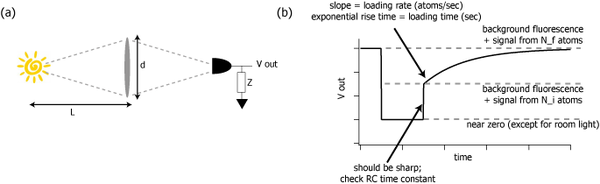
\includegraphics[width=0.9\linewidth]{images/600px-PD3_v2.png}}
    \caption{Photodiode setup for monitoring the number of atoms in the MOT. (a) A fraction of light emitted from the atomic gas is collected by a one-lens optical system and directed onto a biased photodiode, PD3. This fraction is determined by the solid angle $\Omega$ which you determine from the lens diameter $d$ and the distance from the lens to the atomic gas $L$. The photodiode is a current source, so the voltage you observe will depend on the impedance $Z$. This impedance also comprises the capacitance of the photodiode itself (see the \href{http://experimentationlab.berkeley.edu/sites/default/files/images/Photodiode\_info.pdf}{\textbf{spec sheet}}), which determines the effective response time of your photodetector. (b) Operating the ``MOT VI'', you should see a voltage signal similar to the one shown here, from which you can determine the number of atoms in the MOT, $N_i$, once the light is switched back to resonance, the rate $R$ and time constant $\tau$ for loading the MOT, and the steady-state number of trapped atoms $N_f$.}
    \label{fig:600px-PD3_v2}
\end{figure}

Now turn to the triggered CCD camera, which produces a digital image of the MOT, with each pixel now giving a sum of background signal plus the fluorescence due to atoms in a particular location in the MOT. You can determine the number of atoms in the MOT as follows: Take a snapshot, and save the image data. For convenience, you can cut down the size of this file by saving only data within a suitable region of interest (ROI). To determine the total MOT atom number, you might assume the distribution of atoms is Gaussian in the two imaged dimensions, and perform either separate 1D fits (horizontal and vertical) or a single 2D fit to determine the peak intensity and the two rms widths of the Gaussian distribution, and then use these values to derive the integrated atom number over the MOT. Assume that this Gaussian sits atop a smooth background to extract just the signal from the MOT. In principle, you can convert this integrated intensity into an atom number, again using knowledge of the imaging system and the CCD camera settings. However, it's easier just to relate our measurement from the camera to the more easily calibrated photodiode signal.

WARNING: the brightest pixels may be maxed out, and this can distort your measurement. If they are, your camera exposure is too long for this measurement. The procedure for changing the exposure duration is given \hyperref[par:InterfaceToTriggeredCCDCamera]{above}. You will probably want to use the same exposure duration for images at different values of $\delta$.

\begin{itemize}
    \item Obtain a measure of the final MOT number $N_f$ and the MOT size vs. $\delta$, using both the photodiode and the camera, and provide a physical explanation for your results.
\end{itemize}

\subsubsection{Measuring the MOT loading rate}

The equilibrium number of atoms trapped in the MOT is attained when the loading rate of atoms into the MOT, $R $, equals the loss rate. Atoms may be lost from the MOT for several reasons. For example, collisions with high-velocity atoms (e.g. Rb) or molecules (e.g. H$_2$) in the vapor cell can provide an energy to a cold Rb atom that exceeds the MOT trap depth, leading to a loss rate, $N / \tau$, proportional to the number of trapped atoms. At high Rb densities (high MOT atom number), inelastic light-assisted collisions may occur, leading to a loss rate proportional to the square of the density of trapped atoms.

The vapor cell MOT in this experiment is likely dominated by one-body collisional losses, so that one might expect the number of atoms in the MOT to evolve as
\begin{equation}
    \frac{d N}{dt} = R -  N / \tau
\end{equation}
Examining the data from PD3 obtained above for the measurement of the MOT atom number, determine the MOT loading rate $ R $ and MOT-atom lifetime $\tau$ for several settings of the MOT:

\begin{itemize}
    \item At a constant value of $\delta$ and the magnetic field gradient $B^\prime $, vary the size of the MOT laser beams. Can you confirm the expected dependence of the loading rate on the laser beam diameter, \hyperref[subsubsec:CaptureVelocity]{discussed above}?

    \item With the laser beams at maximum diameter, try several settings of $\delta$ and $B'$, describe the trends that you observe and explain them based on the underlying physics.

    \item Is our model for the rate of change of the MOT atom number correct? Provide a quantitative answer. For this, you might perform a $\chi^2$ test, or, you might amend the equation above with an additional loss term, $- \beta N^2$, and ascertain whether the data indicate a significant non-zero value for $\beta$.
\end{itemize}

\subsubsection{Measuring the MOT temperature}
\label{subsubsec:MeasuringMOTTemperature}

What is the lowest temperature you've ever experienced? Even in the coldest climate, you're very unlikely to have been colder than 10's of degrees below 0 C (273 K). Maybe you've made ice cream with liquid nitrogen (at 77 K) or even been fortunate enough to work with liquid helium (4 K). To get colder yet, you might resort to a helium-4 refrigerator (around 1 K) or even a helium-3 dilution refrigerator ($>$10 mK).

Laser cooling has been used to reach some of the lowest temperatures ever. Your task here is to measure the temperature of atoms in your MOT. To measure their temperature, we will attempt to make a measurement of the velocity distribution of atoms in the MOT, which, for an ideal gas at thermal equilibrium, is given by the Maxwell-Boltzmann distribution. To make this measurement, we start with a MOT at equilibrium, and then suddenly switch off the MOT so as to allow the atoms to expand ballistically for a set time of flight, $t_\text{TOF}$. We then make a measurement of the size of the cold-atom gas by one of two means described below.

To carry out this measurement, we make use of the ``MOT VI'' again. To switch off the MOT, we use the shutter placed just after the EOM to extinguish the laser light quickly. After $t_\text{TOF}$, we open the shutter, suddenly reintroducing the laser light. Note: ideally, we would also switch the MOT current off and on again so that the atoms truly propagate freely during the time of flight. The remaining magnetic fields can exert forces on the atoms, due to their magnetic dipole moment.

\begin{itemize}
    \item Consider an ideal gas of particles with mass $m$ with a spherically symmetric, 3D Gaussian density distribution defined by the rms radius $\Sigma$, and with a spatially uniform, thermal distribution (at temperature $T$) of velocities. If you wish, you can consider this as a gas at equilibrium in an external potential that rises as $r^2$ where $r$ is the distance from the origin. At time $t = 0$, the gas is suddenly allowed to expand ballistically (meaning that your fictitious external potential is suddenly set to zero). At a later time, $t_\text{TOF}$, what is the rms radius $\Sigma(t_\text{TOF})$ of the gas?
\end{itemize}

\textbf{Release-and-catch}

One way to measure the velocity distribution is by counting the number of atoms $N_i$ in the MOT just a few ms after the laser light is returned to resonance, and to interpret this as being the number of atoms that are within the ``capture volume'' of the MOT (the atoms coming out of the MOT should certainly be within the capture velocity). This idea is illustrated in Figure~\ref{fig:600px-PD3_v2}. Without worrying about small multiplicative factors, you might take this volume to be a sphere with radius given by some characteristic dimension of the laser beams.

\begin{figure}[h]
    \centering
    \href{http://experimentationlab.berkeley.edu/sites/default/files/images/400px-Release_catch.png}{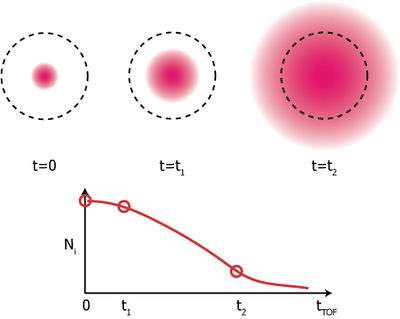
\includegraphics[width=0.5\linewidth]{images/400px-Release_catch.png}}
    \caption{Measuring the MOT temperature by the release and catch method. Before release from the MOT, the atoms (red blob) are held well within the capture volume of the MOT (dashed circle). Note: this is a 2D drawing, but the physics occurs in 3D. After short time of flight ($t = t_1$), the expanding atom cloud is still mostly within the capture volume, so the number of atoms in the MOT once it is switched back on ($N_i$) is still high. After longer time of flight ($t = t_2$), the atom cloud is much bigger than the capture volume, and very few atoms are captured. From the variation of $N_i$ with $t_\text{TOF}$, you can surmise the temperature. However, additional effects limit the reliability of this measurement.}
    \label{fig:400px-Release_catch}
\end{figure}

\begin{itemize}
    \item Using the photodiode monitor, record $N_i$ vs. $t_\text{TOF}$. Use the ``pulse'' function on the VI and be sure that the MOT has sufficient time to fill completely between pulses. Examining the signal on PD3, you should record both $N_i$ and $N_f$ so that you can adjust your data in case $N_f$ varies during the time you are collecting data. Also, you should determine $t_\text{TOF}$ from the PD3 data trace so that you can account properly for delays in the shutter closing and opening.

    If you examine the PD3 signal for short $t_\text{TOF}$, you will actually see the fluorescence rising in three distinct stages: (1) the level rises very quickly (order 100 microseconds) as the shutter opens, (2) the level rises moderately fast (several ms) as the atoms released from the MOT are gathered again into a new MOT, and (3) the level rises slowly (several 100 ms) as atoms are gathered again from the room temperature vapor. Note this is different than what is shown in Figure~\ref{fig:600px-PD3_v2} (shown for the case where no atoms are re-captured in the MOT).

    \item When you have a satisfactory data set, use it to determine the temperature of the gas. Be sure to explain clearly how you are relating your measurement to the gas temperature.

    \item This release-and-catch method is quite crude, and is susceptible to large errors. In particular, even if the gas were at zero temperature, you would still see $N_i$ decrease with increasing $t_\text{TOF}$ if (i) the atoms emerged from the MOT with a net non-zero velocity, and (ii) as the atoms fall under the force of gravity. Consider these two effects. For (i), what is upper bound on this net velocity set by your data? For (ii), at what non-zero temperature will the variation of $N_i$ vs $t_\text{TOF}$ be dominated by thermal expansion rather than just by gravitational acceleration?
\end{itemize}

\textbf{Time-of-flight imaging}

In fact, the first measurements of the temperature of a MOT, made by the release-and-catch method, greatly overestimated the temperature achieved in the MOT, for some of the reasons you have considered above. To overcome some of these shortcomings, we will try another method to measure this temperature. For this we use the triggered CCD camera, controlled by the ``MOT VI,'' and have it record a snapshot of the atomic fluorescence \emph{right after} the the laser light shuttered back on. If we've done our job right, this fluorescence image will give the distribution of cold atoms before the atoms become deflected by radiation pressure forces of the near-resonant light and gathered back into the MOT.

\begin{itemize}
    \item Record images of the expanding atomic cloud at variable $t_\text{TOF}$. \emph{For each $t_\text{TOF}$ you will have to adjust the delay between the falling edge of the shutter TTL and the CCD image so that you collect the very earliest image of the fluorescing atoms (the delays will be somewhere between 1 and 5 ms).} Note that useful images can be obtained only for short $t_\text{TOF}$ before the fluorescence of atoms released from the MOT becomes invisible against the background fluorescence from the vapor in the chamber.

    \item From each image, determine the central position and the dimensions of the gas, and interpret these data in terms of the initial non-zero velocity of the atoms released from the MOT, their acceleration due to gravity (see note below), and their temperature. You will probably find it convenient to save several images and label the files according to the time of flight.
\end{itemize}

For this task, you will need to know that the camera pixel size is 8.4 $\mu$m $\times$ 9.8 $\mu$m (horizontal $\times$ vertical), and should examine the lenses before the triggered camera to figure out the imaging magnification (it's presently roughly 1/2).

Note that this method is not foolproof. The MOT-trapped atoms are not a Gaussian spatial distribution to start with. The MOT light is not suddenly extinguished and restored; rather the beam intensity (and even its spatial profile) varies in time. The fluorescence from the released atoms is weak, obscured partly by the background fluorescence, and modified owing to the spatially varying Zeeman shifts. Finally, the inhomogeneous magnetic field exerts forces on the atoms during their time of flight.

\textbf{This is a checkpoint and a great time to stop and think about the physics at play. Discuss the following questions with you partner and once you feel you have a better understanding of what is happening, call over a GSI to sign you off:}

Discuss with a GSI or professor about two aforementioned methods of measuring MOT temperature. What are their advantages or disadvantages? Which one is more accurate? What are the errors of measurement?

\subsubsection{Observing optical molasses}

The viscous nature of radiation pressure forces is most evident in optical molasses. Without the confining effects of inhomogeneous Zeeman shifts, the propagation of atoms exposed to counter-propagating red-detuned light is diffusive, rather than ballistic, as described \hyperref[subsubsec:MeasuringMOTTemperature]{above}.

\begin{itemize}
    \item As the last step in this experiment, to see this diffusive expansion, switch off the MOT-coil power supply and watch the subsequent expansion of the cold trapped atoms. Roughly how long does it take for this gas to diffuse beyond the reach of the MOT laser beams?

    \item If you're eager, you can use this visual inspection of optical molasses to determine the diffusion constant for the light-illuminated gas, and compare your result with values derived in the literature based on the atomic physics delineated above.

    \item Last day of the experiment please fill out the \href{\ExperimentEvaluation}{\textbf{Experiment Evaluation}}
\end{itemize}

All Reprints and other information can be found on the \href{http://physics111.lib.berkeley.edu/Physics111/Reprints/MOT/MOT\_index.html}{\textbf{Physics 111 Library Site}}

\begin{thebibliography}{}
\label{sec:References}
    \bibitem{Chu} S. Chu. \href{http://physics111.lib.berkeley.edu/Physics111/Reprints/MOT/Steven\_Chu-Neutral\_Particles.pdf}{\textbf{``Nobel Lecture: The manipulation of neutral atoms,''}} Reviews of Modern Physics 70, 685 (1998).

    \bibitem{Cohen-Tannoudji} C.N. Cohen-Tannoudji. \href{http://physics111.lib.berkeley.edu/Physics111/Reprints/MOT/Cohen-Tannoudji\_RMP\_70-707.pdf}{\textbf{``Nobel Lecture: Manipulating atoms with photons,''}} Reviews of Modern Physics 70, 707 (1998).

    \bibitem{Phillips} W.D. Phillips. \href{http://physics111.lib.berkeley.edu/Physics111/Reprints/MOT/W.Philips_RMP_70-3-1998_p721_1.pdf}{\textbf{``Nobel Lecture: Laser cooling and trapping of neutral atoms,''}} Reviews of Modern Physics 70, 721 (1998).

    \bibitem{Raab} E. Raab, M. Prentiss, A. Cable, S. Chu, and D. Pritchard. \href{http://physics111.lib.berkeley.edu/Physics111/Reprints/MOT/Raab_Prentiss_Chu_PRL_v59-23-1987.pdf}{\textbf{``Trapping of neutral sodium atoms with radiation pressure,''}} Physical Review Letters 59, 2631 (1987).

    \bibitem{Metcalf} \href{http://physics111.lib.berkeley.edu/Physics111/Reprints/MOT/Laser\_Cooling\_and\_Trapping\_HJ\_Metcalf/MOT\%20OCR\%20ch.\%203\%20force\%20on\%20two-level\%20atoms.pdf}{\textbf{5.0}}; \href{http://physics111.lib.berkeley.edu/Physics111/Reprints/MOT/Laser\_Cooling\_and\_Trapping\_HJ\_Metcalf/MOT\%20OCR\%20ch.\%207\%20optical\%20molasses.pdf}{\textbf{5.1}};\href{http://physics111.lib.berkeley.edu/Physics111/Reprints/MOT/Laser\_Cooling\_and\_Trapping\_HJ\_Metcalf/MOT\%20OCR\%20\%20ch.\%2011.4\%20magneto-optical\%20traps.pdf}{\textbf{5.2}} (ch3, 7. 11.4) H.J. Metcalf and P. van der Straten. \href{http://physics111.lib.berkeley.edu/Physics111/Reprints/MOT/Laser\_Cooling\_and\_Trapping\_HJ\_Metcalf/}{\textbf{Laser Cooling and Trapping}} (Springer, 1999).

    \bibitem{Steck} \href{http://physics111.lib.berkeley.edu/Physics111/Reprints/MOT/rubidium85numbers.pdf}{\textbf{``Rubidium 85 D line data''}} and \href{http://physics111.lib.berkeley.edu/Physics111/Reprints/MOT/rubidium87numbers.pdf}{\textbf{``Rubidium 87 D line data''}} Dan Steck, University of Oregon. \href{http://steck.us/alkalidata/}{\textbf{Documents available}}

    \bibitem{Siddons} P. Siddons, C.S. Adams, C. Ge and I.G. Hughes, ``\href{http://physics111.lib.berkeley.edu/Physics111/Reprints/MOT/Absolute\%20absorption\%20on\%20the\%20rubidium\%20D\%20lines-0805.1139v1.pdf}{\textbf{Absolute absorption on rubidium D lines: comparison between theory and experiment,}}'' Journal of Physics B: Atomic, Molecular and Optical Physics 41, 155004 (2008).

    \bibitem{Monroe} C. Monroe, W. Swann, H. Robinson, and C. Wieman. ``\href{http://physics111.lib.berkeley.edu/Physics111/Reprints/MOT/Very\%20Cold\%20Trapped\%20Atoms\%20in\%20a\%20Vapor\%20Cell_PhysRevLett.65.1571.pdf}{\textbf{Very Cold Trapped Atoms in a Vapor Cell.}}'' Physical Review Letters 65, 1571 (1990).

    \bibitem{DiStefano} J.J. DiStefano, A.R. Stubberud, and I.J. Williams. \href{http://physics111.lib.berkeley.edu/Physics111/Reprints/MOT/Schaum's\%20Outline\%20Theory\%20and\%20Problems\%20of\%20Feedback\%20and\%20Control\%20Systems/}{\textbf{Schaum’s outline of theory and problems of feedback and control systems}} (McGraw-Hill; New York; 1990).

    \bibitem{Dorf} R.C. Dorf and R.H. Bishop, ``Modern Control Systems, 8th ed.'', Addison Wesley Longman (1998).

    \bibitem{Bechhoefer} J. Bechhoefer. \href{http://physics111.lib.berkeley.edu/Physics111/Reprints/MOT/Bechhoefer_RMP_v77-2005-p783_1.pdf}{\textbf{``Feedback for physicists: A tutorial essay on control''}} Reviews of Modern Physics 77, 783 (2005)

    \bibitem{Wieman} C.E. Wieman and L. Hollberg. \href{http://physics111.lib.berkeley.edu/Physics111/Reprints/MOT/usingdiodelasersforatomicphysics.pdf}{\textbf{``Using diode lasers for atomic physics''}}, Review of Scientific Instruments 62, 1 (1991). A comprehensive guide to diode lasers

    \bibitem{BSCWriteup} \href{http://socrates.berkeley.edu/~phylabs/bsc/PDFFiles/bscLV-11.pdf}{\textbf{BSC writeup, laboratory \#11}}

    \bibitem{PreciseCriterion} A more precise criterion should be specified for systems that are unstable under open-loop conditions (having poles with positive real parts)

    \bibitem{SUNYStonyBrook} Nicely described in an undergraduate student project from \href{http://laser.physics.sunysb.edu/~simone/mini-project/}{\textbf{SUNY Stony Brook}}

    \bibitem{Corwin} Corwin et al., ``\href{http://physics111.lib.berkeley.edu/Physics111/Reprints/MOT/Frequency-stabilized\%20diode\%20laser\%20with\%20the\%20Zeeman\%20shift\%20in\%20an\%20atomic\%20vapor\%20ao-37-15-3295.pdf}{\textbf{Frequency-stabilized diode laser with the Zeeman shift in an atomic vapor}}'' Applied Optics 37, 3295 (1998).

    \bibitem{Moore} John H. Moore, Christopher C. Davis, Michael A. Coplan, ``\href{http://physics111.lib.berkeley.edu/Physics111/Reprints/MOT/John\%20Moore,\%20Christopher\%20Davis,\%20Michael\%20A.\%20Coplan_Building\%20Scientific\%20Apparatus,\%204th\%20ed.pdf}{\textbf{Building Scientific Apparatus, 4th ed}}'', Cambridge University Press (2009).
\end{thebibliography}

\section{Your Feedback}

This is a new experiment, circa 2009. Now that you have completed this experiment, we would very much appreciate your comments. Please take a few moments to answer the questions below, and feel free to add any other comments. Since you have just finished the experiment it is your critique that will be the most helpful. Your thoughts and suggestions will help to change the lab and improve the experiments. Please be as specific as possible. Thank you!

\begin{itemize}
    \item How was the write-up for this experiment? How could it be improved?

    \item How easily did you get started with the experiment? What sources of information were most/least helpful in getting started? Were the reprints appropriate? Did the Pre-lab discussion help? Did you need to go outside the course materials for assistance? What additional materials could you have used?

    \item What did you like and/or dislike about the experiment?

    \item Would you recommend this lab to fellow student? Why or why not?

    \item What advice would you give to a friend just starting this experiment?
\end{itemize}

\end{document}
